\documentclass[12pt]{book}
\usepackage{mystyle}
\usepackage{hyperref}

% this is to have a new page for each section
\usepackage{titlesec}
\newcommand{\sectionbreak}{\clearpage}

%\DeclareMathOperator{\Tr}{Tr}
%\DeclareMathOperator{\Exp}{exp}
\DeclareMathOperator{\Log}{log}
%\DeclareMathOperator{\Det}{det}
\numberwithin{equation}{section}
\newcommand{\new}[1]{{\color{blue}{#1}}}
\title{NUMERICAL SIMULATIONS OF CONVECTIVE BOUNDARY MIXING FOR ASTROPHYSICAL APPLICATIONS}
\author{Alberto Botto Poala\\
Advisor Prof. Dr. Friedrich Röpke}
\date{07.03.17}
\begin{document}
\renewcommand{\arraystretch}{1.2}

% Upper part of the page. The '~' is needed because \\
% only works if a paragraph has started.
% to set spelling in Vim type :setlocal spell spelllang=en_us

% Author and supervisor

% Bottom of the page


\def\aj{AJ}%
          % Astronomical Journal
\def\araa{ARA\&A}%
          % Annual Review of Astron and Astrophys
\def\arfm{ARFM}%
          % Annual Review of Fluid Mechanics
\def\apj{ApJ}%
          % Astrophysical Journal
\def\apjl{ApJ}%
          % Astrophysical Journal, Letters
\def\apjs{ApJS}%
          % Astrophysical Journal, Supplement
\def\ao{Appl.~Opt.}%
          % Applied Optics
\def\apss{Ap\&SS}%
          % Astrophysics and Space Science
\def\aap{A\&A}%
          % Astronomy and Astrophysics
\def\aapr{A\&A~Rev.}%
          % Astronomy and Astrophysics Reviews
\def\aaps{A\&AS}%
          % Astronomy and Astrophysics, Supplement
\def\azh{AZh}%
          % Astronomicheskii Zhurnal
\def\baas{BAAS}%
          % Bulletin of the AAS
\def\jrasc{JRASC}%
          % Journal of the RAS of Canada
\def\memras{MmRAS}%
          % Memoirs of the RAS
\def\mnras{MNRAS}%
          % Monthly Notices of the RAS
\def\pra{Phys.~Rev.~A}%
          % Physical Review A: General Physics
\def\prb{Phys.~Rev.~B}%
          % Physical Review B: Solid State
\def\prc{Phys.~Rev.~C}%
          % Physical Review C
\def\prd{Phys.~Rev.~D}%
          % Physical Review D
\def\pre{Phys.~Rev.~E}%
          % Physical Review E
\def\prl{Phys.~Rev.~Lett.}%
          % Physical Review Letters
\def\pasp{PASP}%
          % Publications of the ASP
\def\pasj{PASJ}%
          % Publications of the ASJ
\def\qjras{QJRAS}%
          % Quarterly Journal of the RAS
\def\skytel{S\&T}%
          % Sky and Telescope
\def\solphys{Sol.~Phys.}%
          % Solar Physics
\def\sovast{Soviet~Ast.}%
          % Soviet Astronomy
\def\ssr{Space~Sci.~Rev.}%
          % Space Science Reviews
\def\zap{ZAp}%
          % Zeitschrift fuer Astrophysik
\def\nat{Nature}%
          % Nature
\def\iaucirc{IAU~Circ.}%
          % IAU Cirulars
\def\aplett{Astrophys.~Lett.}%
          % Astrophysics Letters
\def\apspr{Astrophys.~Space~Phys.~Res.}%
          % Astrophysics Space Physics Research
\def\bain{Bull.~Astron.~Inst.~Netherlands}%
          % Bulletin Astronomical Institute of the Netherlands
\def\fcp{Fund.~Cosmic~Phys.}%
          % Fundamental Cosmic Physics
\def\gca{Geochim.~Cosmochim.~Acta}%
          % Geochimica Cosmochimica Acta
\def\grl{Geophys.~Res.~Lett.}%
          % Geophysics Research Letters
\def\jcp{J.~Chem.~Phys.}%
          % Journal of Chemical Physics
\def\jgr{J.~Geophys.~Res.}%
          % Journal of Geophysics Research
\def\jqsrt{J.~Quant.~Spec.~Radiat.~Transf.}%
          % Journal of Quantitiative Spectroscopy and Radiative Trasfer
\def\memsai{Mem.~Soc.~Astron.~Italiana}%
          % Mem. Societa Astronomica Italiana
\def\nphysa{Nucl.~Phys.~A}%
          % Nuclear Physics A
\def\physrep{Phys.~Rep.}%
          % Physics Reports
\def\physscr{Phys.~Scr}%
          % Physica Scripta
\def\planss{Planet.~Space~Sci.}%
          % Planetary Space Science
\def\procspie{Proc.~SPIE}%
          % Proceedings of the SPIE
\let\astap=\aap
\let\apjlett=\apjl
\let\apjsupp=\apjs
\let\applopt=\ao

%\maketitle
\new{
%% Titelseiten ähnlich zum Layout des Formulars von der
%% Fakultät für Physik und Astronomie
%%
%% Weitere Infos:
%% http://www.physik.uni-heidelberg.de/aktuelles/studium/
%% (PDF link: ...studium/download/145/Vorlage_Diplomarbeit_Formular.pdf)

%% Titelintro
\thispagestyle{empty}
\begin{center}
  \renewcommand{\baselinestretch}{2.00}
  \Large\sffamily
  Fakult\"{a}t f\"{u}r Physik und Astronomie\\
  \large
  Ruprecht-Karls-Universit\"{a}t Heidelberg
  \par\vfill\normalfont
  Masterarbeit\\
  Im Studiengang Physik\\
  vorgelegt von\\
  Alberto Botto Poala\\
  geboren in Biella, Italy\\
  2017\\
\end{center}
\newpage

%% Titelseite
\thispagestyle{empty}
\begin{center}
  \renewcommand{\baselinestretch}{2.00}
  \Large\bfseries\sffamily
    (Titel)\\
    (der)\\
    (Masterarbeit)
  \par
  \vfill
  \large\normalfont
  Die Masterarbeit wurde von Alberto Botto Poala\\
  ausgef\"{u}hrt am\\
  Heidelberger Institut für Theoretuische Studien\\
  unter der Betreuung von\\
  Herrn Prof. Friedrich R\"{o}pke
  %% Bei externen Masterarbeiten hier noch den zweiten Betreuer einfügen
  %% und den vspace in Z. 45 entsprechend reduzieren
\end{center}\par
\vspace{5\baselineskip}

% Zeilenabstand zurücksetzen
\renewcommand{\baselinestretch}{1.00}\normalsize

%% this will generate title pages similar to the template provided
%% by the Department of Physics and Astronomy Heidelberg
%%
%% More information:
%% http://www.physik.uni-heidelberg.de/aktuelles/studium/
%% (PDF link: ...studium/download/145/Vorlage_Diplomarbeit_Formular.pdf)

%% Titleintro
\thispagestyle{empty}
\begin{center}
  \renewcommand{\baselinestretch}{2.00}
  \Large\sffamily
  Department of Physics and Astronomy\\
  \large University of Heidelberg
  \par\vfill\normalfont
  Master thesis\\
  in Physics\\
  submitted by\\
  Alberto Botto Poala\\
  born in Biella, Italy\\
  2017
\end{center}
\newpage

%% Titlepage
\thispagestyle{empty}
\begin{center}
  \renewcommand{\baselinestretch}{2.00}
  \Large\bfseries\sffamily
    (Title)\\
    (of)\\
    (Master thesis)
  \par
  \vfill
  \large\normalfont
  This Master thesis has been carried out by Alberto Botto Poala\\
  at the\\
  Heidelberg Institute for Theoretical Studies\\
  under the supervision of\\
  Herrn Prof. Friedrich R\"{o}pke
  %% additionally insert second supervisor here if carrying out an
  %% external diploma thesis. Reduce vspace in L. 44 accordingly.
\end{center}\par
\vspace{5\baselineskip}

% reset baselinestretch
\renewcommand{\baselinestretch}{1.00}\normalsize

%% Abstract page
%% =============
%%
%% Content of abstract pages has been put into seperate pages to simplify
%% word counting. Use e.g. the unix command
%%   wc abstract-ger.tex
%% or
%%   wc abstract-eng.tex
%% to get the number of words contained in these files.
\thispagestyle{empty}
\begin{center}
  \begin{minipage}[c][0.48\textheight][b]{0.9\textwidth}
    \small
    \textbf{
    Hydrodynamische Simulationen von Mischungsprozessen über Convective Grenzflächen:
    }\par
    \vspace{\baselineskip}
    %% Latex markup und Zitate funktionieren auch hier
Sogar mit den heute verfügbaren Rechenkapazitäten sind 1D Simulationen, das heißt sphärisch symmetrische Modelle, die einzige Möglichkeit die gesamte Lebensdauer eines Sterns zu simulieren. Obwohl diese Herangehensweise für machne Aspekte extrem erfolgreich war, können einige fundamentale Prozesse wie Konvektion und differentielle Rotation nicht aufgelöst werden. In gewissen Phasen der Sternentwicklung spielt Konvektion eine essentielle Rolle, da sie für die Durchmischung der chemischen Elemente und den Energietransport im Inneren eines Sterns verantwortlich ist. Momentan besteht der einzige Weg, die makroskopischen Effekte von Konvektion in 1D Sternentwicklungsprogrammen zu erfassen, in der Verwendung von parametrisierten Modellen, welche vom Aufbau der Schichten des Sterns abhängen. Es würde einen Meilenstein der Sternentwicklung darstellen, wenn man eine konvektive Grenzschicht nur mit Hilfe von Hamilton'schen und hydrodynamischen Variablen charakterisieren und ihr zeitliches Verhalten vorhersehen könnte. In dieser Arbeit wurde eine differentielle Studie des Problems der Durchmischung an konvektiven Grenzschichten anhand von mehrdimensionalen hydrodynamischen Simulationen durchgeführt. Es wurden verschiedene Schichtungen des Fluids sowie konvektive Geschwindigkeiten getestet und die daraus folgende Durchmischung an der Grenzschicht ausgewertet.

  \end{minipage}\par
  \vfill
  \begin{minipage}[c][0.48\textheight][b]{0.9\textwidth}
    \small
    \textbf{
    Hydrodynamic Simulations of Convective Boundary Mixing:
    }\par
    \vspace{\baselineskip}
    %% Latex markup and citations may be used here
(abstract in english, at most 200 words. Example: \cite{loremIpsum})
\new{
The only way to simulate the entire lifespan of a star, even with the current computational resources, is through 1D simulations, i.e.\ by simulating spherically symmetric objects. Although this approach has been for some aspects extremely successful, some fundamental processes as convection and differential rotation are not resolved. Convection plays a primary role in certain evolutionary stages of stars, being one of the responsible for chemical mixing and energy transport in the stellar interiors. The only way to currently map the macroscopic effects of convection in 1D stellar evolution codes in through parametrized models that are stratification-dependent. A milestone in stellar evolution would be to characterize a general convective boundary by means of hamiltonian and thermodynamical variables only and predict its behavior over time. In this work a differential study of the convective boundary mixing problem (CBM) was carried out, by means of multidimensional hydrodynamic simulations. Different fluid stratifications and convective velocities were tested, and the consequent boundary mixing were measured.
}

  \end{minipage}
\end{center}

}
\tableofcontents
%%%%%%%%%%%%%%%%%%%%%%%%%%%%%%%%%%%%%%%%%%%%%%%%%%%%%%%%%%%%%%%%%%%%%%%%%%%%%%%%%%%%%%%%%
% SECTION INTRODUCTION
%%%%%%%%%%%%%%%%%%%%%%%%%%%%%%%%%%%%%%%%%%%%%%%%%%%%%%%%%%%%%%%%%%%%%%%%%%%%%%%%%%%%%%%%%


\chapter{Introduction}
Nature is known for having three mechanisms to transport heat.  

The first one is through \textbf{heat conduction}. Suppose we have two identical bricks of iron at two different temperatures and we could look at the atomic scale, the only difference we would notice is that the atoms of the warmer brick shake more. To say it in a more rigorous way, their mean kinetic energy (with a random velocity) is higher, hence so is the thermal energy. Imagine we put the two bricks in contact, the atoms of the warmer would start to hit and bounce off the atoms of the colder, transferring thermal energy (or heat) from the one to the other, until they reach a situation of equilibrium. This is of course the \textbf{Zero Law of Thermodynamics}. 

The second mechanism is \textbf{radiation}. Every object with a non-zero absolute temperature emits a black body radiation, as long as atomic bounding configurations are complex enough in order to allow the application of the Boltzmann statistics for the energetic distribution of electrons (this is true for objects that have a number of atoms on the order of the Avogadro Number, and even far less). This allows a body to lose thermal energy over time through emission of electromagnetic radiation. This is the mechanism through which Earth and other planets re-emit the radiation received by the Sun and reach thermodynamic equilibrium (it cannot happen through conduction, since this would require that molecules in the atmosphere transfer their thermal energy to molecules or atoms in space, which are too rarefied to allow this). 

The third mechanism, which is the topic of this thesis, is \textbf{convection}. If we consider a fluid stratification like in the atmosphere in which certain thermodynamic conditions are fulfilled, the medium might become unstable in certain regions and give rise to macroscopic ascending and descending blobs which later decay to smaller scale blobs and finally into turbulence. This enables a very efficient transfer of quantities such as heat and chemical composition through different layers of the fluid stratification. 

A \textit{Cumulonimbus}, the typical cloud of thunderstorms, is a perfect example of such a phenomenon. They seldom reach an altitude higher that ten thousand meters because thermodynamical conditions for convection are generally prohibitive in these regions of the atmosphere. Nevertheless when a convective blob hits the stable layer, two phenomena happen. First its turbulent motion erodes mass from it and over time the convective boundary moves upward. Second the hit of the blob imprints an internal mode in the stable layer. These two are the reasons for which planes avoid flying not only into thunderstorms but also above them, because they expect to find turbulence. 

These phenomena happen also in stellar inertia. A convective region over time entrains mass from the stable one, mixing energy and chemical composition (and hence affecting nuclear reaction rates) and imprints internal modes that can be observed on stellar surfaces (the field that studies this phenomenon is asteroseismology, which relies on data of space observatories such as \textit{KEPLER}). It is therefore of fundamental importance to model the dynamics of the convective boundary and the \textbf{Convective Boundary Mixing} (CBM) problem, in order to properly understand stellar evolution. This is the ultimate goal of this work.


%%%%%%%%%%%%%%%%%%%%%%%%%%%%%%%%%%%%%%%%%%%%%%%%%%%%%%%%%%%%%%%%%%%%%%%%%%%%%%%%%%%%%%%%%
% SECTION UNDERLYING PHYSICS
%%%%%%%%%%%%%%%%%%%%%%%%%%%%%%%%%%%%%%%%%%%%%%%%%%%%%%%%%%%%%%%%%%%%%%%%%%%%%%%%%%%%%%%%%

\chapter{Underlying Physics}
\section{Hydrodynamics}
As with all the most beautiful and successful laws of Physics, Hydrodynamics is derived from some conserved quantities. 

The following derivation of the equations of hydrodynamics, which are the foundation for our simulations, is inspired to the one presented by M. Bartelmann in \textit{Theoretical Astrophysics} \cite{theoastro}. 
\subsection{Derivation of the Equations of Ideal Hydrodynamics}

Let's consider for instance a monoatomic gas in a box. A fundamental assumption in ideal hydrodynamics is that the mean free path of particles is infinitesimal. Particles might be spatially equally distributed (like in a bottle) or might not (maybe because the box is so big that we get a density stratification like in the atmosphere). The same concept holds for the velocity distribution: it might be Maxwellian or it might not be. 
In any case we can define the \textbf{distribution function in phase space} $f( \vec{x^{\mu}}, \vec{p^{\mu}})$ such that

$$N=\int \ d^4x \ d^4p \ f( x^{\mu}, p^{\mu}) \  \delta_D[(p^0)^2-\vec{p}^2+m^2c^2] \  \Theta(p^0)$$ 
 where $N$ is the total number of particles, $\delta_D$ is the Dirac $\delta$ function that selects in the integrations only the hypersurfaces physically allowed by the energy-momentum relation of General Relativity, and finally $\Theta$ makes sure that we are taking into account only positive momenta. 
Keeping this in mind, we can define the first and second momenta of our distribution function

\begin{align}
J^{\alpha}= c \int \frac{dp^3}{E} \ f( x^{\mu}, p^{\mu}) p^{\alpha}  &&   T^{\alpha \beta}= c \int \frac{dp^3}{E} \ f( x^{\mu}, p^{\mu}) p^{\alpha}p^{\beta}  
\end{align}
 
namely the \textbf{current density} $J$ and the \textbf{energy-momentum tensor} $T$. Carrying out the calculation the components read 


\[
  J= \frac{n(t,\vec{x})}{c}
  \begin{pmatrix}
    c \\
    \left< \dot{x} \right> \\
    \left< \dot{y} \right> \\
    \left< \dot{z} \right> \\
  \end{pmatrix}\quad
  T= \rho(t,\vec{x})
  \begin{pmatrix}
    c^2 \left< \gamma \right> & c \left< \gamma \dot{x} \right> &  c \left< \gamma \dot{y} \right> & c \left< \gamma \dot{z} \right> \\
     c \left< \gamma \dot{x} \right> & \left< \gamma \dot{x}^2 \right> &  \left< \gamma \dot{x}y \right> &  \left< \gamma \dot{x} \dot{z} \right>  \\
     c \left< \gamma \dot{y} \right> &  \left< \gamma \dot{y} \dot{x} \right>&  \left< \gamma \dot{y}^2 \right> &  \left< \gamma \dot{y} \dot{z} \right>  \\
     c \left< \gamma \dot{z} \right> &  \left< \gamma \dot{z}\dot{x} \right>& \left< \gamma \dot{z}\dot{y} \right> &  \left< \gamma \dot{z}^2 \right> 
  \end{pmatrix}
\]

where $n(t, \vec{x})$ is the number density, $c$ the speed of light,  $\left< a(t,\vec{x}) \right>$ means the average of the quantity $a$ over time and space in a neighborhood of $(t, \vec{x})$, $\gamma$ is the well known general relativistic parameter.

By integrating the first and second momentum of Boltzmann Equation, one can show that $J$ and $T$ are divergenceless, meaning in the non-relativistic case
\begin{align}
\frac{\partial }{\partial^{\mu}}J^{\mu}=0 && \frac{\partial }{\partial^{\mu}}T^{\mu \nu}=0 \  \  \forall \nu =0,..,3 
\end{align}
This means that if we apply the operator $(c^{-1}\partial_t,\partial_x,\partial_y,\partial_z)$ to $J$ and $T$ we equal zero. Doing so with the density current we obtain the \textbf{continuity equation}
\begin{equation} \label{cont}
\partial_t \rho + \vec\nabla \cdot (\rho \vec{v})=0
\end{equation}
We then apply the same procedure to the energy-momentum tensor.

We might choose to do it in the first column ($\nu=0$), and that would lead us to the \textbf{energy conservation equation}
\begin{equation} \label{consen}
\partial_t \epsilon + \vec \nabla \cdot (\epsilon \vec{v}) + P\vec \nabla \cdot \vec{v}=0
\end{equation}
where $\epsilon$ is the internal energy and $P$ the pressure. These two variables, that were not explicitly included in $T$, arise naturally by splitting up the microscopic velocity of the fluid $\left <  \dot{x} \right >$ into a mean macroscopic velocity $\vec{v}$ and a random velocity $\vec{u}$ in the neighborhood of the mean one. 
$$\left <  \dot{x} \right >= \vec{v}  +  \vec{u} $$
and recalling that 
$$\epsilon = \frac{\rho}{2} \left <  u^2 \right > = \frac{3}{2} n k_B T= \frac{P}{2}$$
When we operate on the other three columns of $T$, we obtain the \textbf{momentum conservation equations} for the three spatial dimensions.
\begin{equation} \label{euler}
\partial_t \vec{v} + (\vec{v} \cdot \vec \nabla) \vec{v} + \frac{\vec \nabla P}{\rho}=0
\end{equation}
These last three are often called \textbf{Euler equations}. 

Note that the operator on the left hand side is nothing but the total time derivative
$$
\partial_t + \vec{v} \cdot \vec \nabla = \frac{d}{dt}
$$
so what we are actually writing is Newton's equation per unit volume
$$
\rho \vec{a} = \vec \nabla P
$$
In case other macroscopic forces like gravity are present, we simply add them on the right hand side as we would do in classical mechanics. 

So far we have obtained 5 equations in 6 unknowns, namely the internal energy $\epsilon$, the momentum $\vec{p}$, the pressure $P$ and the density $\rho$. If we want to have at least a chance of integrating the system we're missing one equation, the \textbf{equation of state}, that relates the thermodynamic variables.

\subsection{Viscous Hydrodynamics}

As stated at the beginning of the previous section, one fundamental assumption of ideal hydrodynamics is that particles have an infinitesimal mean free path. What actually happens in nature might be very different. Particle have a finite mean free path, and hence they can transport local properties all through the fluid by diffusion: transport of energy generates heat conduction, transport of momentum friction. The consequence is that we end up with one additional term in the energy-momentum tensor representing the diffusive processes
$$
T^{ij} \to T^{ij} + T^{ij}_d 
$$

The density current remains unchanged (hence continuity equation) because mass is always conserved. As in the previous subsection, the new energy-momentum tensor needs to be operated on with $\nabla$ and set equal to zero in order to obtain our modified equations in the viscous case. We will not carry out all the calculations, rather simply quote the result for the viscous versions \ref{consen} and \ref{euler}. 

The new energy conservation equation reads
$$
\partial_t \epsilon + \vec \nabla \cdot (\epsilon \vec{v}) + P \vec \nabla \cdot \vec{v} = \vec \nabla \cdot (k \vec \nabla T) + v_{ij} T_d^{ij} 
$$
where $v_{ij}$ is the symmetrized velocity gradient tensor
$$
v_{ij} = \frac{1}{2}(\partial_i v_j + \partial_j v_i)
$$
This equation shows that the internal energy in a certain region of the fluid can change either if there is a temperature gradient or if the fluid is moving with a velocity field with a non vanishing symmetrized gradient (non solid-body rotation) because of friction.
The new momentum conservation equations read
$$
\rho \left( \partial_t + \vec{v} \cdot \vec \nabla \right) v^j+\partial^jP = \eta \vec \nabla^2v^j + \left( \xi + \frac{\eta}{3} \right) \partial^j \vec \nabla \cdot \vec{v}
$$
These are often called \textbf{Navier-Stokes Equations}, and thoroughly show the nonlinearity of hydrodynamic.

\subsection{Hydrostatic Equilibrium in Stars}
We shall now consider the static configuration of \ref{euler} with gravitational potential. This reads
\begin{equation} \label{hystat}
	\vec \nabla P = - \rho \vec \nabla \Phi
\end{equation}
This shows that the pressure stratification is adjusted only by the shape of gravity. We can say more by taking the curl of this equation and we get
$$
\vec \nabla \rho \times  \vec \nabla \Phi =0
$$
which shows that the gradient of the gravitational potential and of the density are parallel. Surfaces of constant density are surfaces of constant gravitational potential.

It is known from classical mechanics that if we are given a spherically symmetric matter distribution, the gravitational acceleration is $g=Gm/r^2$ which leads to
\begin{equation}\label{HydroEquilibrium}
	\frac{\partial P}{\partial r}= - \frac{G m}{r^2} \rho
\end{equation}
The general approach to find the relation between the pressure and the density consists in taking the divergence of \ref{hystat} and substituting the Poisson equation 
$$
\vec \nabla \cdot \left ( \frac{\vec \nabla P}{\rho} \right ) = - 4 \pi G \rho 
$$
This equation can be solved only if an equation of state (EoS) is provided. For instance if we choose a polytropic equation of state (which means that the pressure is a function of the density only and not of the temperature) we obtain the \textbf{Lane-Emden Equation} that allows stable solutions for adiabatic indices up to $4/3$ only. This EoS is used for instance for modeling white dwarfs, where the pressure doesn't depend on the temperature because of the degeneracy of the gas. 

\section{Energy Transfer}
\new{
	The present chapter about energy transfer and the following one about convection are inspired to the work of Kippenhahn, Weigert and Weiss \textit{Stellar Structure and Evolution} \cite{stellarstruc}.
}
\subsection{Transport of Energy by Radiation}
In the deep interiors of stars energy is generated through nuclear reactions. In the Sun for instance all the energy is provided by hydrogen burning into helium (the so-called p-p chain), while just a little fraction by virialization. Because temperature is of the order of $10^9 K$, thermal motions allow protons to overcome the electrostatic potential barriers and interact through the nuclear force, giving rise to the reaction
\begin{equation}\label{ppchain}
	6 \mathrm{H}^1 \to \mathrm{He}^4_2 + 2 \mathrm{H}^1 + 2 \gamma + 2 \nu
\end{equation}
where on the right hand side we have photons and neutrinos, that carry energy away. 

Neutrinos, interacting only via the weak force, have a very low cross section and hence leave the core of the sun without scattering, draining energy very efficiently. We need to take into consideration very massive systems like Core Collapse Supernovae and Neutron Stars in order to see a tangible interaction between the neutrino flux and matter. These astronomic objects are actually excellent neutrino laboratories provided by nature. 

Photons instead, interacting electromagnetically, scatter multiple times before reaching the \textit{photosphere}, the region where statistically they scatter for the last time before ending up in our eyes or our telescopes. 

Let's now make a rough estimate of the mean free path of a photon in the sun. 
\begin{equation}\label{mfp}
	l_{p,p}=\frac{1}{k \rho}
\end{equation}
where $k$ is the mean cross section (averaged over all frequencies) per unit mass. For ionized hydrogen in stellar medium a rough average is $1 \ cm^2/g$. The average density of the sun is $\bar\rho_{\odot}=3M_{\odot}/4 \pi R_{\odot}^3= 1.4 \mathrm{g /cm}^3$. 

Plugging in the numbers we get $\bar l_{p,p \odot}=2 \  \mathrm{cm}$. 

At this point we need to answer a fundamental question: do two sequential scatterings happen at thermodynamic equilibrium? In other words when one photon scatters, and then scatters again a few millimeters or centimeters away, does it encounter the same thermodynamic conditions? In order to evaluate that, let's consider the mean temperature gradient between the center of the sun and the photosphere
$$
\frac{\Delta T}{\Delta r} = \frac{10^7 \ \mathrm{K}-10^4  \ \mathrm{K}}{R_{\odot}} \simeq 1.4 \times 10^{-4} \  \mathrm{K} \ \mathrm{cm} ^{-1}
$$
which means that after $2 \mathrm{cm}$ on the radial direction a photon sees a difference in temperature of $\Delta T = l_{p,p} \times 1.4 \times 10^{-4}  \  \mathrm{K} \ \mathrm{cm} ^{-1}= 3 \times 10^{-4} \  \mathrm{K}$. The relative difference of radiation energy density can be easily computed since $u \sim T^4$, hence in the center of the sun $\Delta u/u=4 \Delta T / T \sim 10^{-10}$: between two scatterings a photon is in \textbf{Local Thermodynamic Equilibrium} (LTE). This little anisotropy that we neglect is the actual cause of the luminosity of the sun, because it generates a non-vanishing net flux.
\subsection{Diffusion of radiative energy}
We have seen that the mean free path $l_{p,p}$ of photons is much smaller that the characteristic length of our physical system, hence we are allowed to treat the scattering processes statistically. This leads us to describe energy transfer as a diffusion process. 

The diffusive flux $j$ of a certain species of particles (number of particles migrating per unit area and unit time) is given by
\begin{equation}\label{diffusion}
	\vec  j=-D \nabla n
\end{equation}
where $n$ is the species density. $D$ is the diffusion coefficient
\begin{equation}
	D =\frac{1}{3} v l_{p}
\end{equation}
which is a function of the mean free path and of the mean velocity. What we are actually interested in is not the diffusive flux of the particles $j$, but rather in the diffusive flux of their energy $\vec F$. The density needs to be substituted with the energy density $u=aT^4$, $\bar v$ with $c$ and $l_p$ with $l_{p,p}$. $a$ is the radiation density constant. If we assume spherical symmetry the gradient of $u$ is simply the radial component
\begin{equation}
	\frac{\partial u}{\partial r} = 4  a  T^3   \frac{\partial T}{\partial r}
\end{equation}
So recalling \ref{diffusion} we have immediately that
\begin{equation}
	F=-\frac{4ac}{3}\frac{T^3}{k \rho} \frac{\partial T}{\partial r}
\end{equation}
which can be written down in a more compact way as 
\begin{equation}
	\vec F = - k_{rad} \nabla T
\end{equation}
after having properly defined $k_{rad}$ as the conduction coefficient. Now we use the well known relation between luminosity and flux and solve it for the temperature gradient
\begin{equation}
	\frac{\partial T}{\partial r}= - \frac{3}{16 \pi a c}\frac{k \rho l}{r^2 T^3}
\end{equation}
which in lagrangian coordinate reads
\begin{equation}\label{partialTpartialm}
	\frac{\partial T}{\partial m}= - \frac{3}{64 \pi^2 a c}\frac{k l}{r^4 T^3}
\end{equation}
We should never forget the assumptions we made when deriving this equation, namely the LTE. When we approach the photosphere, for instance, the density decreases, the mean free path increases, and two scattering events happen so far away that LTE doesn't hold any longer. In this case radiation transport is no more a diffusive process. 

Another form of heat transfer is conduction, but in stellar physics it becomes relevant only in cores of red giants or white dwarfs and it is fully neglected in our simulations.

\subsection{The astrophysical $\nabla$}
Assuming hydrostatic equilibrium we can now divide \ref{partialTpartialm} by \ref{HydroEquilibrium} in lagrangian coordinates and obtain
\begin{equation}
	\frac{\partial T/\partial m}{\partial P / \partial m} = \frac{3}{16 \pi a c G} \frac{k l}{m T^3}
\end{equation}
This is nothing but the derivative of the temperature with respect to the pressure, which increasing monotonically upward, is representative of the radius. We furthermore rewrite this quantity as
\begin{equation}\label{nablarad}
	\nabla_{\mathrm{rad}} = \left( \frac{d \ln T}{d \ln P}  \right)_{\mathrm{rad}}= \frac{3}{16 \pi a c G} \frac{k l P}{m T^4}
\end{equation}
This quantity will be of fundamental importance when we will discuss convective stability. Recall that we took into account only radiative transfer, but defining $k$ properly we could take into account also heat conduction.
\section{Fundamental Equations of Stellar Structure}
At this point we are able to write down a system of equations that we will call \textbf{fundamental equations of stellar structure}, which describe a simplified but still very useful model. This will hold in a static, stable and spherically symmetric case.

\textbf{Mass continuity} 

Here $m(r)$ is the mass contained inside the sphere of radius $r$
\begin{equation}\label{masscons}
	\frac{dm}{dr}=4 \pi r^2 \rho
\end{equation}

\textbf{Hydrostatic equilibrium} 

We have already encountered the hydrostatic equilibrium equation
\begin{equation}\label{hydroeq}
	\frac{dP}{dr}= - \frac{G m(r)}{r^2} \rho
\end{equation}

\textbf{Equation of State} 

So far we have written down two equations in three variables, namely $m$, $\rho$, and $P$. If we want to have at lest a chance to solve them we need another equation, namely the equation of state. Possible choices are:
\begin{itemize}
	\item $\rho=const$ this would be the case for liquids.
	\item $P\propto \rho^\gamma$ i.e.\ the density and pressure are not a function of the temperature. This is the case, as already stated in the previous section for white dwarfs and leads to the Lane-Edmen equation and its solutions.
	\item $P=\frac{\mu}{R}\frac{P}{T}$ the equation of state for perfect gases and it's the case for the sun. It has the inconvenience that it introduces another variable, namely the temperature $T$, and hence it doesn't solve our original problem. We need at least another equation to solve the system. 
\end{itemize}

\textbf{Energy conservation} 

In case we have an energy source (such as nuclear reactions), this needs to be conserved
\begin{equation}\label{energycons}
	\frac{dL}{dr} = 4 \pi r^2 \epsilon
\end{equation}

\textbf{Temperature gradient} 

Of crucial importance to understand convection will be the following equation for the astrophysical nabla
\begin{equation}\label{energytransfer}
\frac{d T}{d r} = - \frac{T }{P} G m \rho\nabla
\end{equation}


\section{Convection}
Until now we have assumed a perfect spherical symmetry, meaning that all dynamical and thermodynamical quantities were a function of the radius only. Obviously this is not a realistic case. For a number of reasons stars have small perturbations, that may eventually grow and give rise to macroscopic phenomena. A classic example is convection.

We are relaxing the spherically symmetric case, but this doesn't mean that our fundamental equations of stellar structure are useless. As explained in the introduction, if we could section stars we would see that convection appears in concentric regions, hence  we can still treat the problem as spherically symmetric, defining dynamic and thermodynamical quantities as averages on a proper region. 

We shall now understand when, given thermodynamic variables, we are dealing with a dynamically stable or unstable layer.


\subsection{Dynamical instability}
Let's consider a perfect density stratification like the one in a star or in the atmosphere and let's break the symmetry of the system by adding a little perturbation in the thermodynamic variables. For any given quantity $A(r, \theta)$ (from now on $A_e$, because it's a function of the mass element we are considering), we compute $A_s$ (which is an average at given $r$ on the surrounding material). We can assume that the fluid moves adiabatically, thus the timescale for heating transfer is much smaller than the timescale for convection turnover. 

We define a local property of the fluid 
$$
DA=A_e - A_s
$$
For instance we could imagine that a little region of a star is slightly hotter than the surroundings, hence we have in that region $DT > 0$. Note that because of the assumption we have made $DP=0$ always, because when these is a pressure spike, the gas expands at the sound velocity $c_s$ which is way higher than the low hydro regime we observe in stellar inertia.

If we have a $DT>0$, since in a perfect gas the equation of state reads $\rho \sim P/T$, we obtain $D \rho < 0$. With a lower density, that mass element will be lifted by buoyancy. In a non adiabatic workframe it might happen that heat is exchanged so quickly that temperature differences vanish immediately, but we assumed adiabatic processes. The question we are trying to answer is if the mass element, after a little upward movement, will still be buoyant and give rise to macroscopic convection, or if it will bounce back. The answer lies obviously in the temperature gradient, i.e.\ if once lifted a little bit the new $DT$ will still be in favor to buoy it to the next layer, and so on. 

Let's approach the problem from another point of view. Let's assume that we have a stable layer without perturbations, and we lift a mass element upward of $\Delta r$. The density difference now is
\begin{equation}\label{eq:displacement}
D \rho = \left [  \left( \frac{d \rho}{d r} \right)_e - \left( \frac{d \rho}{d r} \right)_s   \right ] \Delta r
\end{equation}
where the first derivative tells us how much the density of the mass element changes when lifted, the second one tells us how the surrounding density changes along the radial direction. 

We call the buoyancy force per unit volume 
$$
f_b=- g \ D \rho
$$
which points upward if $D \rho < 0$, which is the unstable configuration. If instead $D \rho > 0$ the mass element sinks back to its original position and no macroscopic motion appears. As a consequence $D \rho<0$ is our \textbf{condition for stability}.

The problem with this criterion is that very often the density gradient is not known, since it does not appear in the fundamental equations for stellar structure. In order to proceed let's turn our gradient in spacial coordinate into a gradient in thermodynamic coordinates. As previously stated, our transformations are adiabatic, hence no exchange of energy occurs. This is very close to reality for stellar inertia. To begin let's write down the equation of state $\rho = \rho (P, T, \mu)$ in a differential form
\begin{equation}\label{eq:EoSdiff}
	\frac{d \rho}{\rho} = \alpha \frac{d P}{P} - \delta \frac{d T}{T} + \phi \frac{d \mu}{\mu}
\end{equation}
where $d \mu$ represents the change in the chemical composition, including ionization processes. 

Substituting \ref{eq:displacement} in \ref{eq:EoSdiff} we obtain
\begin{equation}
	\left (\frac{\alpha}{P} \frac{dp}{dr}\right )_e - \left ( \frac{\delta}{T}\frac{dT}{dr}\right )_e -  \left (\frac{\alpha}{P} \frac{dp}{dr}\right )_s +  \left ( \frac{\delta}{T}\frac{dT}{dr}\right )_s -  \left ( \frac{\phi}{\mu}\frac{d \mu}{\mu dr}\right )_s>0 
\end{equation}
The two terms containing the pressure gradient cancel each other out because as previously stated $DP=0$. Let's multiply the remaining terms by the so called \textbf{pressure scale height} $H_P$
\begin{equation}\label{scaleheight}
	H_P=-\frac{dr}{d \ln P}= - P \frac{dr}{dP}
\end{equation}
$H_P$ has the dimension of a length, being the characteristic distance over which the pressure changes.
We finally obtain our condition for stability
\begin{equation}\label{criterionstab}
	\left (   \frac{d \ln T}{d \ln P}    \right )_s <  \left (   \frac{d \ln T}{d \ln P}   \right )_e +  \frac{\phi}{\mu} \left (   \frac{d \ln \mu}{d \ln P}    \right )_s
\end{equation}
We have already encountered the first term which is $\nabla_{rad}$ of \ref{nablarad}.
Let's define two new quantities
\begin{equation}\label{nablas}
	\nabla_{e} = \left (  \frac{d \ln T}{d \ln P}   \right )_e \  \nabla_{\mu} = \left (  \frac{d \ln \mu}{d \ln P}   \right )_s
\end{equation}
Recall that since pressure is always decreasing at increasing radius we can measure the temperature as a function of the pressure, and hence its gradient. Furthermore, since our mass element buoys adiabatically, we call $\nabla_e=\nabla_{\mathrm{ad}}$. 
With this new notation we can write down our stability criterion in a more compact way as
\begin{equation}\label{stabcritcomp}
	\nabla_{\mathrm{rad}} < \nabla_{\mathrm{ad}} + \frac{\phi}{\delta} \nabla_{\mu}
\end{equation}
and obtain the \textbf{Ledoux criterion}. 

In our simulations we used a monoatomic ideal gas equation of state, hence $\nabla_{\mu}=0$.  What we obtain is the \textbf{Schwarzschild criterion} for dynamic stability
\begin{equation}\label{schwarzschild}
	\nabla_{\mathrm{rad}}<\nabla_{\mathrm{ad}}
\end{equation}
If the left hand side is bigger than the right hand side, it means that our stratification is not able to transport all the energy generated only through radiation, and it is hence required to rely on convection. 

Note that up until now we simply have found a stability criterion, but we don't know anything about the convection that will arise. In the next section we will try to quantify it, especially since we need to know how much energy is transported from one layer to the other in order to map this result in 1D simulations of stellar evolution.

\subsection{Mixing length theory}
A fundamental problem in stellar astrophysics is to understand how much energy is transported by convection. Before the era of computational physics, when only analytics solutions were available, the most common tool used to model convective energy transport was the so called \textbf{mixing length theory} (Böhm-Vitense 1958). 

The total energy flux $l/4 \pi r^2$ at given radius is given by the radiative flux $F_{\mathrm{rad}}$ (which may also include the conductive flux), and the convective flux $F_{\mathrm{con}}$. Their sum is according to \label{nablarad} what defines the $\nabla_{\mathrm{rad}}$ that would be necessary to transport away all the energy.
\begin{equation}\label{7.1}
F_{\mathrm{rad}}+ F_{\mathrm{con}}= \frac{4 a c G T^4 m }{3 k P r^2} \nabla_{\mathrm{rad}}
\end{equation}
But part of it is ultimately transported by convection, at the most $\nabla_{\mathrm{rad}}$ can equal $\nabla$. 
\begin{equation}\label{7.2}
F_{\mathrm{rad}}= \frac{4 a c G T^4 m}{3 k P r^2} \nabla
\end{equation}
In order to quantify then $F_{\mathrm{con}}$, let's consider a blob with a $DT$ over its surroundings. Its motion will be mainly radial which a velocity $v$ and with $DP=0$ for reasons already explained. We can write down the energy flux as
\begin{equation}\label{fconv}
	F_{\mathrm{con}}=\rho  v  c_P  DT
\end{equation}
Of course we should average $v$ and $DT$ over an imaginary sphere and hence obtain an equation that holds statistically over the solid angle at a given radius and not locally. One can deduce since now the approximations and limits of this theory. 

Bulbs have an initial velocity that equals zero, and the same holds for $DT$. Over time it will migrate a distance $l_m$, namely the \textit{mixing length} before dissolving via turbulent cascade. This means that on average a bulb will move a distance $l_m/2$ where it accelerates, and another $l_m/2$ where it decelerates the same amount to stop at the end of the convective zone. Bulbs will definitely also change shape during the migration, which makes it pretty difficult to strictly define temperature and velocity, but in a very rough approximation we claim that
\begin{equation}
	\frac{DT}{T}=\frac{1}{T}\frac{\partial (DT)}{\partial r} \frac{l_m}{2}=(\nabla-\nabla_e)\frac{l_m}{2}\frac{1}{H_P}
\end{equation}
which is simply a Taylor expansion to determine $DT$ after $l_m/2$. Recall that the buoyancy force per unit mass is $f_b=-g \cdot D \rho / \rho$ and that $D \rho / \rho - \delta D T / T$. Let's pretend on average that half of this force acting on the blob during its migration of $l_m$, hence the work done is
\begin{equation}\label{7.6}
	\frac{1}{2} k_r \frac{l_m}{2}=g \delta (\nabla - \nabla_e)\frac{l_m^2}{8 H_P}
\end{equation}
Let's furthermore suppose that only half of this work ends up in kinetic energy, because the other half has to go in the work necessary for moving the surroundings. Then the average velocity of an element half way is
\begin{equation}
	v^2=g \delta (\nabla - \nabla_e)\frac{l_m^2}{8 H_p}
\end{equation}
and plugging this result into \label{fconv}
\begin{equation}
F_{\mathrm{con}}= \rho c_P T \sqrt{g \delta} \frac{L^2_m}{4\sqrt{2}}H_P^{-3/2} (\nabla-\nabla_e)^{3/2}
\end{equation}
Now let's consider a sphere of diameter $d$ slightly hotter than the surrounding and moving radially with velocity $v$. It will lose energy because of radiative processes and because of the adiabatic expansion. The energy lost in time due to the first process is
\begin{equation}
\left (\frac{d E}{d t}  \right )_{\mathrm{rad}} = \frac{8 a c T^3}{3 k \rho} DT \frac{S}{D}
\end{equation}
hence the drop in temperature per unit length radially, taking into account both processes is
\begin{equation}\label{7.7}
	\left (  \frac{d T}{d r }   \right )_e = \left(  \frac{dT}{d r }   \right )_{\mathrm{rad}} - \frac{\left( d E / dt \right)_{\mathrm{rad}} }{\rho V c_P v}
\end{equation}
Which multiplied by $H_P/T$ gives
\begin{equation}
\nabla_e - \nabla_{\mathrm{ad}} =  \frac{\left( dE/dt \right)_{ \mathrm{rad} } H_P}{\rho V c_P v T}
\end{equation}
Plugging in the expression that we derived for $(dE/dt)_{\mathrm{rad}}$ and taking an average for $DT$, we are left with an equation that contains a "form factor" $l_m S/Vd$ that for a sphere should of course be $6/l_m$. In the literature $9/2l_m$ it's often used instead and this brings us to
\begin{equation}\label{7.11}
\frac{\nabla_e - \nabla_{\mathrm{ad}}}{\nabla - \nabla_e} = \frac{6acT^3}{k \rho c_P l_m v}
\end{equation}
We finally obtained five equations(\ref{7.1}, \ref{7.2}, \ref{7.6}, \ref{7.7}, \ref{7.11}) in five variables ($F_{\mathrm{rad}}$, $F_{\mathrm{con}}$, $v$, $\nabla_e$, $\nabla$). Note that the mixing length $l_m$ is not one of those variables, and hence is a free parameter for which we have to assume a value. 

Although the mixing length theory has been used extensively in 1D stellar evolution, in many occasions it has been proven unsuccessful, especially because of the uncertainties about the parameters (Viallet \emph{et al.} 2015, Georgy \emph{et al.} 2016). Thanks to the rise of computational resources over the last decade, atmospheric scientists and astrophysicists were able to run 2D and 3D Hydro simulations and approach the problem more heuristically. They concluded that the controlling parameter for the boundary migration could be the \textbf{bulk-Richardson number}, which is the topic of the next section.  


\subsection{Bulk-Richardson Number}

So far we got to the point where we have a convective layer and a stable layer above or beneath it. What happens over time is that the convective boundary entrains mass from the stable layer by ingestion, because turbulent eddies capture stable fluid that is consequentially dragged and entrained in the turbulent layer. A fundamental problem in stellar evolution is to understand the dynamics of this boundary: what is its velocity (if we are in an eulerian workframe), or how much mass from the stable layer is entrained in unit time (in a Lagrangian workframe).

One of the methods used to model the migration is the bulk-Richardson number
\begin{equation}\label{bulkrichardson}
	\mathrm{Ri}_{B}=\frac{\Delta b L}{\sigma_t^2}
\end{equation}
which is a dimensionless parameter that compares the strength of the boundary to the one of the turbulence. $L$ is the length scale of the turbulence (which is definition dependent), $\sigma_t$ is the standard deviation of its velocity, $\Delta b$ is the so called buoyancy jump between unstable and stable layer.

In our case we define the length scale of the turbulence $L$ as follows. Let's consider the autocorrelation function 
\begin{equation}\label{correlation}
	a(\Delta r)= \langle f(r) f(r + \Delta r) \rangle
\end{equation}
where the brackets mean average over all possible $r$, but at fixed correlation length $\Delta r$. Recall that such a function always has a maximum for $\Delta r=0$, (because every function $f$ is perfectly equal to itself), then $a(\Delta r)$ decreases with increasing $\Delta r$ (because $f(r+\Delta r)$ resembles less and less $f(r)$ as $\Delta r$ increases). If $f$ is periodic with period $T$, then the autocorrelation function $a$ has maximum with periodicity $T$. In order to define $L$ we autocorrelate the mach number in the horizontal direction of the convective region and take the length at which $a$ drops to a half of its maximum, i.e. \ $a(L)/a(0)=0.5$.

The buoyancy jump is defined by considering the \textbf{Brunt-Väisälä frequency} 
\begin{equation}
	N^2(r)=-g \left (  \frac{\partial \ln \rho}{\partial r} -  \frac{\partial \ln \rho}{\partial r} \Big|_{s}  \right )
\end{equation}
and integrating it over the boundary
\begin{equation}
	\Delta b = \int_{r_i}^{r_f} N^2 dr
\end{equation}
Of course we need a proper definition of the boundary limits $r_i$ and $r_f$. In our case we defined them by initializing a passive scalar in the convective region, which is over time advected in the unstable layer. By looking at the gradient of the concentration of the passive scalar in the vertical direction, one notices two spikes, which represent the boundary positions at given $\mathrm{x}$. By averaging over $\mathrm{x}$ and by computing the standard deviation, we are able to define the boundary positions and their width.

Let's furthermore define the \textbf{entrainment coefficient} $E$ as the boundary migration speed $u_b$ over the turbulence standard deviation $\sigma$. Previous works have found that
\begin{equation}
	E=A \mathrm{Ri}_{B}^{-n}
\end{equation}
Where $A$ and $n$ are coefficients that need to be determined, and this will be the primary goal of our simulations.

In a Lagrangian workframe this transforms to
\begin{equation}
	\dot{M}_\mathrm{E}=\frac{\partial M}{\partial r} u_E
\end{equation}
If this relation is proven to be true, it would be possible to know the boundary migration speed $u_b$ or the mass entrainment rate $\dot{M}_\mathrm{E}$ given only $L$, $\Delta b$ and $\sigma_t$, and consequentially map this phenomenon into 1D stellar models. In the hope that these two free parameters exist and are universal (i.e. \ not system-, code- or resolution-dependent), the goal of this work is to determine them and to test their universality.


%%%%%%%%%%%%%%%%%%%%%%%%%%%%%%%%%%%%%%%%%%%%%%%%%%%%%%%%%%%%%%%%%%%%%%%%%%%%%%%%%%%%%%%%%
% SECTION RECENT WORKS 
%%%%%%%%%%%%%%%%%%%%%%%%%%%%%%%%%%%%%%%%%%%%%%%%%%%%%%%%%%%%%%%%%%%%%%%%%%%%%%%%%%%%%%%%%

\chapter{Previous works}

\section{Numerical simulations}

The only way to study thoroughly the macroscopic effects of convection like the boundary mixing problem is through multidimensional simulations. Only in the last decade computational power allowed astrophysics groups to run 3D simulations with a satisfying resolution. We report here what we believe are the most significant works carried out in the past. 

\paragraph{Turbulent Convection in Stellar Interiors I. Hydrodynamic Simulation. \textit{Meakin et al}, 2007.} 
The first extensive work was carried out by C. Meaking and D. Arnett (2007) who simulated the oxygen shell burning and the hydrogen core burning in a $23 M_{\odot}$ star both in 2D and in 3D, using the "box in a star" approach. In the core burning simulation they had only one boundary to analize, during the shell they had both the superior and inferior. This group used the 1D stellar evolution code TYCHO that was then mapped into PROMPI, a multidimensional parallelized hydro code that solves euler equations implementing PPM (piecewise parabolic method) with a nuclear reaction network. They reported $\log A=0.027 \pm 0.38$ and $n=1.05 \pm 0.21$ for the three dimensional case. \\
As we have seen in the previous section, the definition of the bulk-Richardson number is model dependent. In this case in order to define the boundary and its topology, they injected a passive scalar in the convective region. The biggest drop in its concentration defined the boundary topology. They then computed the mean value of the boundary coordinate and its standard deviation, which delimited the initial and final position of the convective boundary over which integrate the Brunt-Väisääla frequency in order to obtain the buoyancy jump. They furthermore defined the length scale of the turbulence as the length where the autocorrelation of the mach number drops below $0.5$. This is a simple but effective set of definitions and procedures that I used in my data analysis too. \\
\paragraph{3D Hydrodynamic Simulations of Carbon Burning in Massive Stars. \textit{Cristini et al}, 2016.} 
Another recent study has been carried out by A. Cristini et al, 2016. They simulated a Carbon burning shell in a $15 M_{\odot}$ star (box in a star method) spanning around $3000$ s and $2 \times 10^9$ cm in four runs with different resolutions (from $128^3$ to $1024^3$). They used the same code PROMPI with self gravity in the Crowling approximation necessary to describe deep interiors of stars, and they used a very similar procedure to get the entrainment rate coefficient. After analyzing the convective structure with help of the Reynolds-averaged Navier-Stokes equations (RANS), they reported parametric values of $A= 0.06 (+0.27 / -0.04)$ and $n= 0.81 (+0.38 / -0.28)$. Although the second one agrees pretty well with the previous study, the first one is not even in the same order of magnitude and affected by huge uncertainty, hence the motivation for this work.

\chapter{Code Description}
\section{Code Overview}
The code we used is called Seven League Hydro (SLH). It was originally developed by Dr.\ Fabian Miczek during his PhD thesis (Miczek, 2013). SLH is a finite-volume multidimensional code that solves the Euler equations (ideal hydrodynamic) using explicit or implicit time discretization.

The code automatically decomposes the domain to parallelize the computation on the desired number of processors on distributed memory (MPI) and shared memory enviroments (OpenMP). A wide choice of boundary conditions are implemented. 

Furthermore SLH implements a general equation of state, a nuclear reaction network, passive and active scalars which are fundamental for the study of the chemical composition of the fluid, radiation in the diffusion limit and thermal conduction. 

Over the years SHL has undergone several scaling tests, the most remarkable of which at the Jülich Supercomputing Center (JSC) in 2016 where it scaled over all the $458752$ cores of \textit{JUQUEEN} (a Blue Gene machine, currently the latest generation of IBM supercomputers).

\section{Finite Volume Discretization}
This chapter follows section 3.3 of Miczek (2013).

In order to discretize the physical domain we employ a set of curvilinear coordinates $\xi, \eta, \zeta$. This set is partitioned by a regular, equidistant grid with $N_{\xi} \times N_{\eta} \times N_{\zeta}$ cells. Without loss of generality, we define the domain extent such that
\begin{equation}
\begin{split}
\xi \in [1/2, N_{\xi} + 1/2] \\
\eta \in [1/2, N_{\eta} + 1/2] \\
\zeta \in [1/2, N_{\zeta} + 1/2] 
\end{split}
\end{equation}
Here we impose that the cell volume is constant, i.\ e.\ $\Delta \xi = \Delta \eta = \Delta \zeta = 1$ in order to simplify some calculations. This may, in general, not be the case, since SLH allows the user to call a general curvilinear grid. In this particular with this notation integer values of coordinates refer to the centers of the cells, half integer to cell faces, e.\ g.\ by $(\xi, \eta, \zeta) = (i, j + 1/2, k)$ we refer to the interface at the right-hand side of cell $(i, j, k)$.

Both for analytic and numerical study of Euler equations, it is useful to switch to a dimensionless workframe. This is achieved by decomposing state variables into two parts, namely a reference value (denoted with an $r$) and a dimensionless number (denoted with a hat), e.g. $\rho = \rho_r \cdot \hat{\rho}$. This leads to equations for the state vector 
\begin{equation}
\frac{\partial \mathbf{\hat{U}}}{\partial \hat{t}} + \frac{\partial \mathbf{\hat{F}}_x}{\partial \hat{x}} + \frac{\partial \mathbf{\hat{F}}_y}{\partial \hat{y}} + \frac{\partial \mathbf{\hat{F}}_z}{\partial \hat{z}} = \mathbf{\hat{S}}
\end{equation}
where the quantities $\mathbf{\hat{U}}$, $\mathbf{\hat{F}}_x$, $\mathbf{\hat{F}}_y$ and $\mathbf{\hat{F}}_z$ are defined by the stress-energy tensor as discussed in the previous chapter. From now on for simplicity we will drop the hat notation. We discretize the spatial component of in space Euler equations as 
\begin{equation}
J^{-1}\frac{\partial \mathbf{U}}{\partial t} + \nabla_{\xi, \eta, \zeta} \cdot \mathbf{F} = J^{-1} \mathbf{S}
\end{equation}
where $J$ is the determinant of the Jacobian of the transformation from the physical domain to the computational grid.

These equations are integrated over the volume $\Omega_{i, j, k} = \Delta \xi \times \Delta \eta \times \Delta \zeta $ of the cell $i, j, k$, which in our assumptions is constant for every cell (differentially $d \Omega = d \xi \times d \eta \times d \zeta$) of the cell $(i, j, k)$. The integrals read
\begin{equation}
	\int_{\Omega_{i, j, k}} J^{-1} \frac{\partial \mathbf{U}}{\partial t} d \Omega + \int_{\Omega_{i, j, k}} \nabla_{\xi \eta \zeta} \cdot \mathbf{F} d\Omega = \int_{\Omega_{i, j, k}} J^{-1} \mathbf{S} d \Omega
\end{equation}

By exchanging the derivatives with the integrals, it is clear that these are nothing but the average of the conserved quantities in the cell times the volume of it. We may therefore introduce some new cell-averaged quantities such as 
\begin{equation}
\mathbf{U}_{i, j, k} = \int_{\Omega_{i, j, k}} J^{-1} \mathbf{U} d \Omega \qquad \mathbf{S}_{i, j, k} = \int_{\Omega_{i, j, k}} J^{-1} \mathbf{S} d \Omega
\end{equation}
In addition to this, we can apply Gauss theorem on the second term on the left-hand side and obtain the following expression
\begin{equation}
	\frac{\partial \mathbf{U}_{i, j, k}}{\partial t} + \frac{1}{V_{i, j, k}} \oint_{\partial \Omega} \mathbf{F} \cdot d \mathbf{s} = \mathbf{S}_{i, j, k}
\end{equation}
If we suppose to know the integral fluxes through the six interfaces, we can further decompose the second term into six numerical fluxes as follows
\begin{equation}
\begin{split}
	\mathbf{F}_{i+ 1/2, j, k} = \oint_{\partial \Omega_{(i + 1/2, j, k)}} \mathbf{F}_{\xi} d \xi \\
	\mathbf{F}_{i, j + 1/2, k} = \oint_{\partial \Omega_{(i , j + 1/2, k)}} \mathbf{F}_{\eta} d \eta \\
	\mathbf{F}_{i, j, k + 1/2} = \oint_{\partial \Omega_{(i , j, k + 1/2)}} \mathbf{F}_{\zeta} d \zeta \\
\end{split}
\end{equation}
This allows us to write down the discretized Euler equations as 

\begin{equation}
\begin{split}
	\frac{\partial \mathbf{U}_{i, j, k}}{\partial t} + \frac{1}{V_{i, j, k}} ( & \mathbf{F}_{i + 1/2, j, k} + \mathbf{F}_{i - 1/2, j, k} +\mathbf{F}_{i , j + 1/2, k} + \\
	& \mathbf{F}_{i , j - 1/2, k} +  \mathbf{F}_{i , j, k + 1/2} + \mathbf{F}_{i , j, k - 1/2}) = \mathbf{S}_{i, j, k}
\end{split}
\end{equation}
What is stored in the memory are the cell-averaged quantities. Their value changes only by numerical fluxes from the neighbor cells or by source terms. This implies that if there are no source terms, the sum of cell-averaged variables cannot change (except for fluxes across the boundaries). In this way, the finite volume discretization perfectly reflects the conservative nature of hydrodynamic. We would like to emphasize that the numerical fluxes still remain unknown, and should be reconstructed for the cell $(i, j, k)$ from the surrounding interfaces. 

In addition to that, what we performed was a \textit{partial discretization}, since we still have a continuous time derivative and no finite difference. This method, through which we discretize first the spatial dimension and then separately the temporal one, is known as the \textbf{method of lines}. It is a very effective method to reduce partial differential equations to a set of coupled ordinary differential equations such as
\begin{equation}\label{eq:methodoflines}
	\frac{\partial \mathbf{U}_{i, j, k}}{\partial t} + \mathbf{R}_{i, j, k}=0
\end{equation}
where the vector $\mathbf{R}_{i, j, k}$ is known as \textit{spatial residual} of the cell $(i, j, k)$. As previously mentioned, this is a function with the numerical fluxes of the surrounding cells, and suitable numerical methods are needed in order to correctly compute them.
\section{Explicit vs. Implicit Time Stepping}
This follows sections 5.1 and 5.2 of Miczek (2015).

The simplest way to discretize in time equation \ref{eq:methodoflines} is the so called \textbf{forward Euler method} \footnote{The forward Euler method can be applied to resolve general PDEs, not only Euler equations. It is a coincidence that both the fluid dynamics equations and the numerical scheme that we use to solve them were discovered by Swiss mathematician Leonhard Euler.}:
\begin{equation}\label{eq:forwardeuler}
	\frac{\mathbf{U}^{n+1}_{i, j, k} - \mathbf{U}^{n}_{i, j, k}}{\Delta t} + \mathbf{R}_{i, j, k}(\mathbf{U}^n)=0
\end{equation}
This method simply approximates the time derivative with a finite difference at each grid point, and a spacial residual is evaluated at the old time step. Notice that equation \ref{eq:forwardeuler} can be solved analytically for the conserved quantity $\mathbf{U}^{n+1}_{i, j, k}$. This means that we are dealing with an \textit{explicit time stepping}. Although equation \ref{eq:forwardeuler} has a very direct and simple implementation, this method is accurate to firstorder i.e.\ it has an approximation error that is $\mathcal{O}(\Delta t)$.

A considerable amount of higher-order explicit time stepping schemes are available. In SLH the a third-order Runge-Kutta scheme (RK3) developed by Shu and Osher (1988) is implemented. 

There are essentially two advantages of an explicit time stepping method: they are easy to implement and they require little resources memory-wise on the hardware. The biggest disadvantage is that one always has to choose the time step lower than a maximum value $\delta t$. In case this condition is not fulfilled, numerical errors start to grow over time and dominate over the physical solution. In the case of Euler equations, in order to determine $\delta t$, the CFL criterion is generally used:
\begin{equation}\label{eq:cfl}
	\Delta t = \frac{\mathrm{CFL}}{N_{\mathrm{dim}}}\mathrm{min} \left(  \frac{\Delta x}{|q_n| + c/M}   \right)
\end{equation}
where $N_{\mathrm{dim}}$ is the number of dimensions, $\Delta x$ is the cell width, the quantity in denominator is the wave velocity and the minimum has to be evaluated over all the computational grid. At last CFL is a dimensionless coefficient that determines how many cells a wave can travel for time step. For all the explicit time steppers implemented in SLH, CFL is always smaller than unity. One can see that, roughly, $\Delta t \propto M$, hence the lower the mach number, the lower the maximum allowed time step. This criterion shows why the use of explicit time steppers for low mach flow is computationally impracticable.
For this reason we rely on a new discretization method, namely the \textbf{backward Euler method}. According to this discretization the conserved quantities at the time step $n+1$ are given by
\begin{equation}\label{eq:backward}
	\frac{\mathbf{U}^{n+1}_{i, j, k} - \mathbf{U}^{n}_{i, j, k}}{\Delta t} + \mathbf{R}_{i, j, k}(\mathbf{U}^{n+1})=0
\end{equation}
The only difference compared to the forward Euler method is that the residual is evaluated at the time step $n+1$ instead of $n$. An analytic solution for this equations is, in general, not possible, and sophisticated numerical solvers need to be employed in order to find an approximate solution (in our case we implement the so-called \textbf{Newton-Raphson method}, see next section). The advantage of integrating implicitly is very well explained by figure \ref{fig:implicit}. What is shown is a slow advection wave with a relatively low frequency, with a high frequency acoustic wave on it. Suppose we start integrating from $t=0$ explicitly with the forward Euler method. Since the derivative is evaluated at $t=0$, the risk is that the acoustic wave completely dominates the result, leading to a corrupted value for the conserved quantity. Integrating implicitly instead, the derivative is evaluated over the entire time step. In other words we extrapolate the derivative starting from the final point backward to the initial one, ensuring that the finite difference method resolves the phenomena at the time scale we are interested in. Acoustic waves in the low mach regime in fact decouple from the advective solution, hence we don't need to resolve them. The backward Euler method again generates an error which is $\mathcal{O}(\Delta t)$, but more refined methods are available in the literature and are implemented in SLH. 

\begin{figure}[t]
\centering
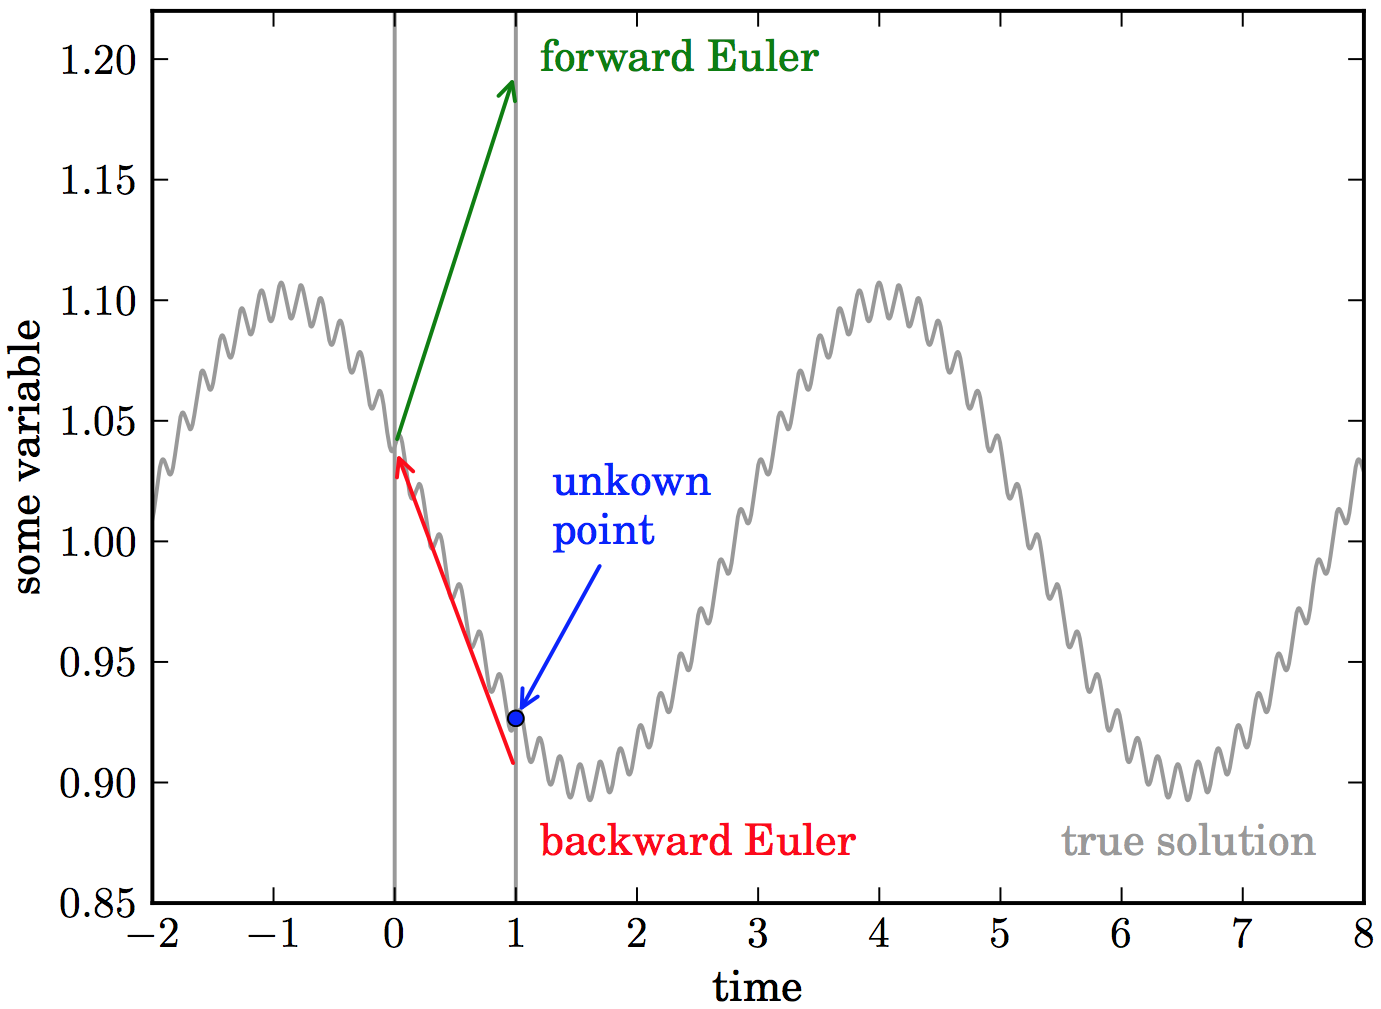
\includegraphics[width=10cm]{./img/implicit}
\caption{Conceptual difference between explicit and implicit integration. Picture from Miczek, 2013.}
\label{fig:implicit}
\centering
\end{figure}
The question we need to answer when choosing the integration technique is if the rise in efficiency given by implicit methods compensate the loss, given by the expensive numerical solvers needed to approximate the solution of the implicit equation. In the low mach regime (from $M \simeq 10^{-4}$ to $10^{-3}$) an implicit integration with SLH is always more convenient. 

\section{Newton-Raphson Method}
In this section we analyze the so-called \textbf{Newton-Raphson method}, which is the iterative solver implemented in SLH in order to find an approximate solution to the implicit equation \ref{eq:backward}. 

The first step we need to take is to move every term of our discretized equation to the left-hand side and define a quantity $\mathbf{D}_{i, j, k}(\mathbf{U}^{n+1})$ called the \textit{defect}:
\begin{equation}\label{eq:defect}
	\mathbf{D}_{i, j, k}(\mathbf{U}^{n+1}) = \mathbf{R}_{i, j, k}(\mathbf{U}^{n+1}) + \frac{\mathbf{U}_{i, j, k}^{n+1}}{\Delta t} - \frac{\mathbf{U}^n_{i, j, k}}{\Delta t} = 0
\end{equation}
Obviously the equations are solved if the defect is zero. This algorithm starts from an initial guess $\mathbf{U}^0$, which is iteratively refined by calling
\begin{equation}\label{eq:newtonraphson}
	\mathbf{U}^{k+1} = \mathbf{U}^k - \left( \lambda \frac{\partial \mathbf{D}^k}{\partial \mathbf{U}}  \right)^{-1} \mathbf{D}^k
\end{equation}
Where $\lambda$ is a convergence parameter that in generally set to one (in pathological cases it might be set $\lambda > 1$ to dump the convergence ratio). The more the iterations, the closer $\mathbf{U}^k$ gets to the root of $\mathbf{D}$.

In order to compute the right-hand side, one should invert the Jacobian of the defect, but this is computationally and memory-wise very expensive. It is instead easier to rewrite \ref{eq:newtonraphson} as 
\begin{equation}
	\lambda \frac{\partial \mathbf{D}^k}{\partial \mathbf{U}} \Delta \mathbf{U} = - \mathbf{D}^k
\end{equation}
where $\Delta \mathbf{U}=\mathbf{U}^{k+1} - \mathbf{U}^k$. This is a very effective method to transform a system of non-linear equations to a set of systems of linear equations.

The Newton-Raphson method generally converges quadratically to the solution, i.e.\ the number of significant digits doubles at every iteration. In particular cases like a double root (namely $f'(\alpha)$=0, where $\alpha$ is the defect root) the convergence is linear. Obviously the first and second derivative should be non-zero over the iterative domain and to improve the efficiency the initial guess should be as close as possible to the root of the defect. In SLH we choose as $\mathbf{U}^0$ the solution of the previous time step.

SLH prints in the log file information about every iteration of the Newton-Raphson method for every variable. Specifically it prints the $\mathrm{L2}$ norm of the defect. For the density $\rho$ for instance
\begin{equation}\label{eq:l2defect}
	||\mathbf{D}||^{\rho} = \sqrt{ \sum_{i, j, k} \left( \mathbf{D}^{\rho}_{i, j, k}  \right)^2}
\end{equation}
which is the quantity that decreases quadratically.

In equation \ref{eq:defect} the very last term is a constant vector, since it's the state vector at the previous time step ($t=n$). Only the state vector at the current time step ($t=n+1$) changes at every iteration of the Newton-Raphson method. These sums are of course cause of numerical cancellation errors. In SLH the $\mathrm{L2}$ norm of the defect is scaled by the $\mathrm{L2}$ norm of the constant vector, because different variables have numerically different orders of magnitude.
\begin{equation}
	\frac{||\mathbf{D}||^{\rho}}{||\mathbf{U}^n / \Delta t||^{\rho}}
\end{equation}
This is done in order to monitor the convergence in a dimensionless way and relative to machine precision \footnote{Recall that for double precision floating point value, machine precision is $\simeq 10^{-16}$. }
Note that reaching machine precision when converging is actually rarely possible because of
\begin{itemize}
	\item{round-off errors in the discretization in the flux functions and in the linear solvers}
	\item{approximations in the defect Jacobian and in the linear systems}
\end{itemize}
Moreover, the process of discretization of Euler equations generates errors which depend on the numerical scheme called and the grid chosen. As a consequence, converging to machine precision is often a waste of computational resources.

%%%%%%%%%%%%%%%%%%%%%%%%%%%%%%%%%%%%%%%%%%%%%%%%%%%%%%%%%%%%%%%%%%%%%%%%%%%%%%%%%%%%%%%%%
% SECTION HYDRODYNAMIC SIMULATIONS 
%%%%%%%%%%%%%%%%%%%%%%%%%%%%%%%%%%%%%%%%%%%%%%%%%%%%%%%%%%%%%%%%%%%%%%%%%%%%%%%%%%%%%%%%%

\chapter{Hydrodynamic Simulations}
\section{2D Simulations}
\subsection{Simulations setup}
The physical setup used for our simulations is the so called "box in a star" method, meaning that we simulate some relatively very small internal region of a star. \\
In our case for the 2D runs it will be a box of $2.50 \times 10^{9} cm$ on the $x$ axis and $1.25 \times 10^{9} cm$ on the $y$ axis. Gravity is constant pointing downward on the $y$ axis with a magnitude of $1000 cm/s^2$. This generates a pressure stratification in the fluid that covers approximately three pressure scale heights. \\
The controlling parameter in our setup is the temperature gradient that can be initialized to any value. In our case we divided the simulated region in three parts. The bottom region (labeled as $1$) starts at the lower boundary and reaches $4/12$ of the domain, the central (labeled as $2$) proceeds till the middle, and the upper one (labeled as $3$) reaches the upper boundary, as shown in \ref{fig:tempprofile}. We define a parameter $\alpha_{i}$ ($i=1, 2, 3$) which is nothing but the fraction of the $\nabla$ over the $\nabla_{\mathrm{ad}}$. As seen in previous sections $\alpha_{i}<1$ implies stability in the $i-$region, instability otherwise. \\
We always initialized the setup with $\alpha_{1} = \alpha_{3}$ widely smaller than $1$; and $\alpha_{2}=0.99$, which means a very precarious situation in terms of stability in the second region. A heating function furthermore heats the second region with a Gaussian profile (see \label{fig:tempprofile}) to generate convection that will expand downward and upward by entrainment. The values of $\alpha_{1}$ and $\alpha_{3}$ are controlling parameters for the bulk-Richardson number, since they are proportional to $\Delta b$. The advantage of simulating a strip of convection between two stable layers (miming a Shell convection) instead of a convective region at the bottom that grows upward (Core convection-like) is twofold: it gives us two convective boundaries to study instead of one, and we avoid high mach number at the boundary which can at times generate problems or unphysical situations. \\
One of the hardest tasks has been to generate the correct amount of heating such that the turbulence standard deviation \textit{at the interface} was constant during the run (which is one of the ingredients of the bulk-Richardson number, hence one of the parameters we want to control in order to perform a differential study). In order to do that, the heating function is tuned such that, at $t=100K s$ the total heat generation is reduced to $50 \%$ of the original amount.\\ 
\begin{figure}[t]
\centering
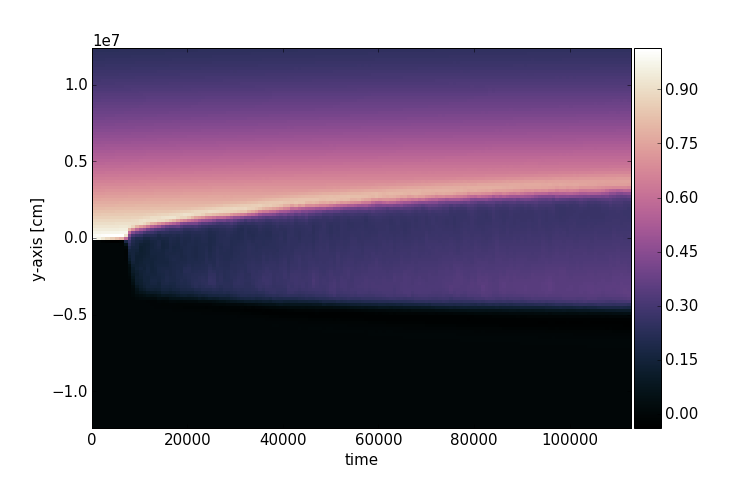
\includegraphics[width=10cm]{./img/tempprofile}
\caption{Example of initial temperature profile along the $y$-axis}
\label{fig:tempprofile}
\centering
\end{figure}
At the bottom of the simulated region small perturbations in temperature and mach number had been imprinted on the stratification in order to break the initial symmetry of the system.\\
A wide range of boundary conditions have been tested for this problem. We used for the horizontal direction periodic boundaries, that definitely provide the most physical situation. For the vertical direction we used wall boundary conditions.\\ 
As briefly explained in the previous sections, in order to define the topology of the convective boundaries, we initialized a passive scalar inside each one of the regions. Recall that passive scalars are just like colors of the fluid and in no way they influence the dynamic of the system, neither they diffuse.\\
As previously stated our goal is to perform a \textit{differential} study of the bulk-Richardson number and the CBM problem. This implies running simulations with different values of $\Delta b$ and $\sigma_t$ at different resolutions. Being 2D simulations computationally so cheap, we managed to run a copious amount of them. With the code 2d0.10-0.80 we will refer to a 2-dimensional run with $\alpha_{1} = \alpha_{3}=0.1$ and $80 \%$ of the heating referring to the arbitrary value of $4.5 10^{15} \mathrm{erg/s}$.\\ 
We run in 2D on a $2048 \times 1024$ uniform Cartesian grid. It is worth remarking that when doing CFD with a higher resolution, one not only resolves better the features of the system, but also decreases the numerical viscosity (increases the Reynolds number). This is the reason for which we chose this grid setup: we want to keep cells squared and keep viscosity a scalar quantity, and prevent it from becoming a tensorial one. In the next section we will perform a convergence study, in order to undertand which roles the resolution and the viscosity play in the phenomenon of convective entrainment.\\ 

\subsection{Evolution of a single run}



\begin{figure}[t]
      \centering
        \subfloat[Mach number profile over time.]{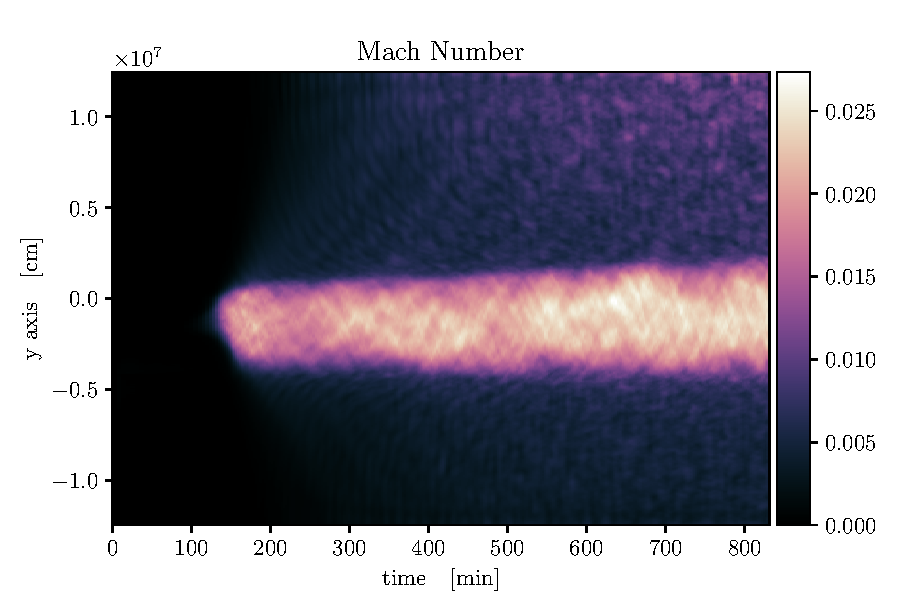
\includegraphics[width=10cm]{./img/mach.pdf}\label{fig:2d0.7-0.01LR.turbmach}}
     \centering
	\hfill
        \subfloat[Entrainment of passive scalar from the upper stable region in the convective region.]{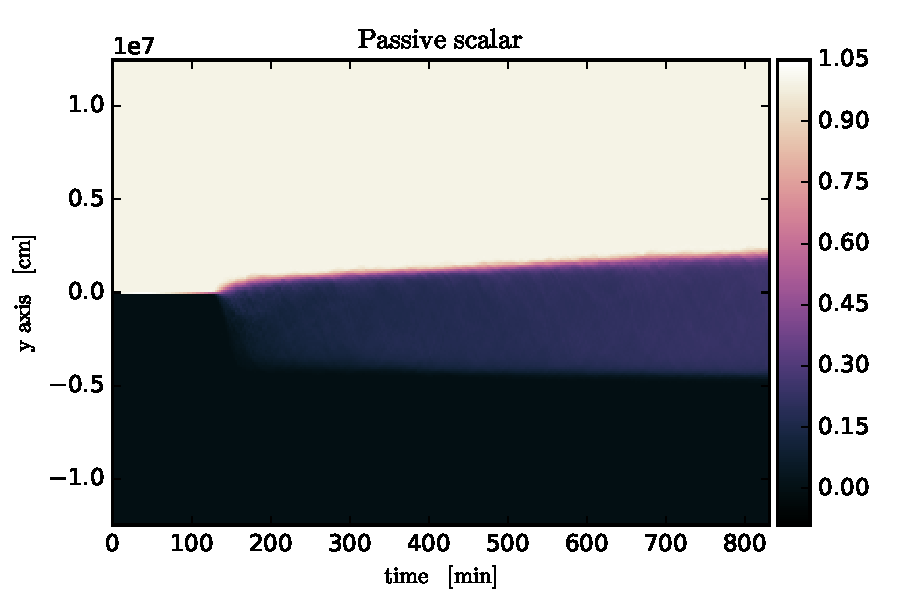
\includegraphics[width=10cm]{./img/ps2.pdf}\label{fig:2d0.7-0.01LR.bp}}
\end{figure}
 %%%%%%%
 % divisione figure %
 %%%%%%%

Let's consider the setup 2d0.10-0.80. \\
Convection starts at around $t \sim 7000 s$. Because of the already mentioned implicit time stepping, the lower the mach number, the bigger the time step, allowing us to save a huge amount of computational resources before the rise of convection. A remarkable difference is also observed in the convective regime, as long as the mach number is below $10 \%$, which has always been our case.\\


In figure \ref{fig:2d001-LRmach} we plot the profile of the mach number over the simulated time. This is what one would expect, with two remarks that need to be done. \\
First of all the mach number is stable over time, thanks to the heating function that we implemented, featuring a decrease of heat generation as previously explained. \\
Second of all it is clear that some internal modes are excited by the convective blobs when they hit the stable layers and they propagate through it. They appear more significant in the upper region and to a certain extent it's true, but mainly this is due to the fact that the speed of sound there it's lower. Plotting the absolute velocity the difference is not so dramatic. Two interesting questions remain without answer. First of all it is impossible to tell to which extent the dynamic of the boundary is influenced by these modes. Second of all it is possible that the chemical mixing due to these modes in the stable stratification might have a significant impact on the evolution of a star, which is obviously not considered in 1-D simulations.\\
\begin{figure}[t!]
  \centering
  \subfloat[Passive scalar avection at the onset of convective motions, at $t \simeq 150 \ \mathrm{min}$]{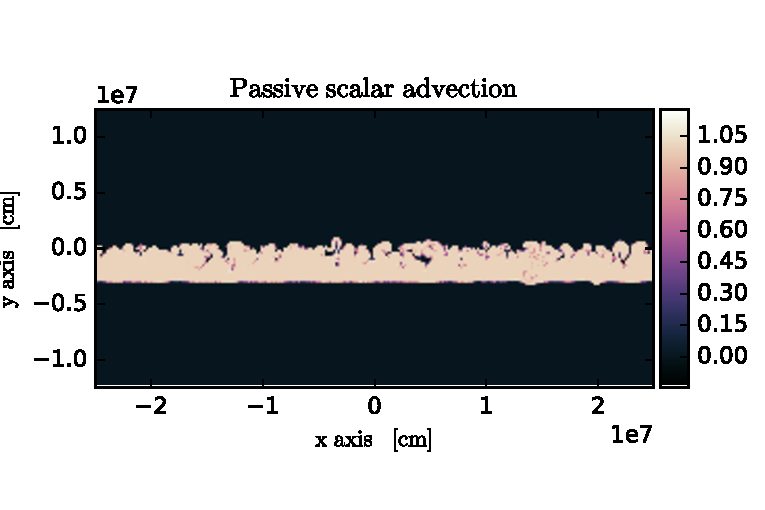
\includegraphics[width=10cm]{./img/passiveacc1.pdf}\label{fig:bulk}}
  \centering
  \hfill
  \subfloat[The same passive scalar of above, advected at $t \simeq 800 \ \mathrm{min}$. This defines the topology of the boundary.]{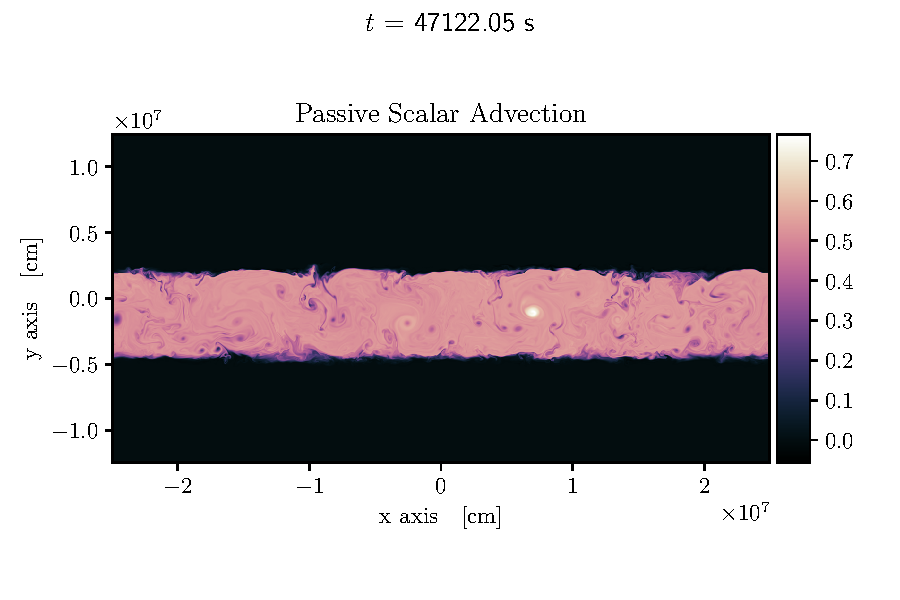
\includegraphics[width=10cm]{./img/passiveacc2.pdf}\label{fig:ent}}
  \end{figure}
In figure \ref{fig:2dsingle} we plot the passive scalar initialized inside the upper region, which over time is entrained by convection. We clearly see the movement of the boundaries that over the $60000 s$ of simulated time move gradually upward and downward. Specifically in the upper case it starts in the middle of the simulated region and ends up at $\sim 7.0 \times 10^{6} cm$, for the lower case it starts at $\sim 3.7 \times 10^{6} cm$ and moves downwards to the middle of the simulated region \\
In figure \ref{fig:2dsingle} we plot some parameters relevant to our analysis. \\
\begin{figure}[t!]
  \centering
    \subfloat[Bulk-Richardson number over time.]{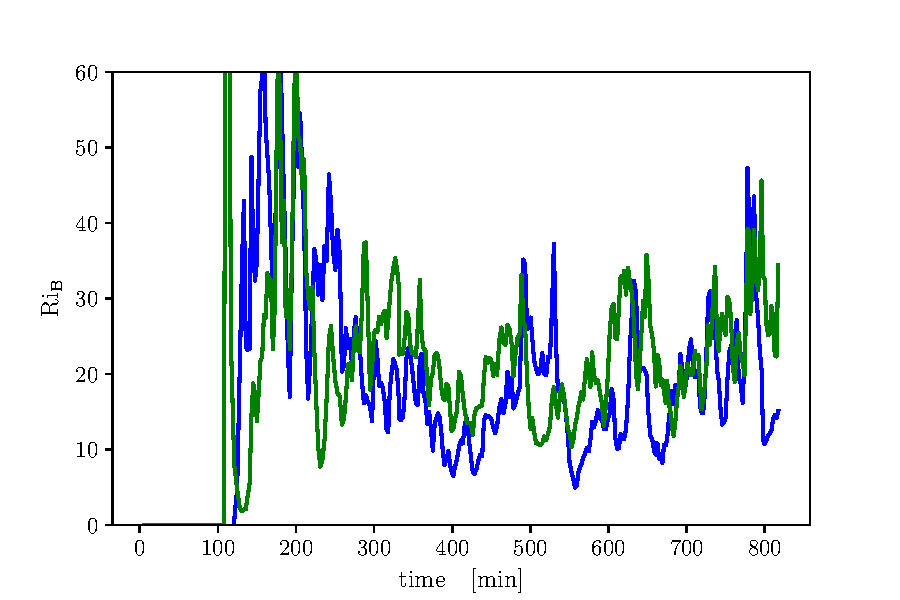
\includegraphics[width=0.5\textwidth]{./img/bulk.pdf}\label{fig:bulk}}
      \hfill
        \subfloat[Entrained mass over time.]{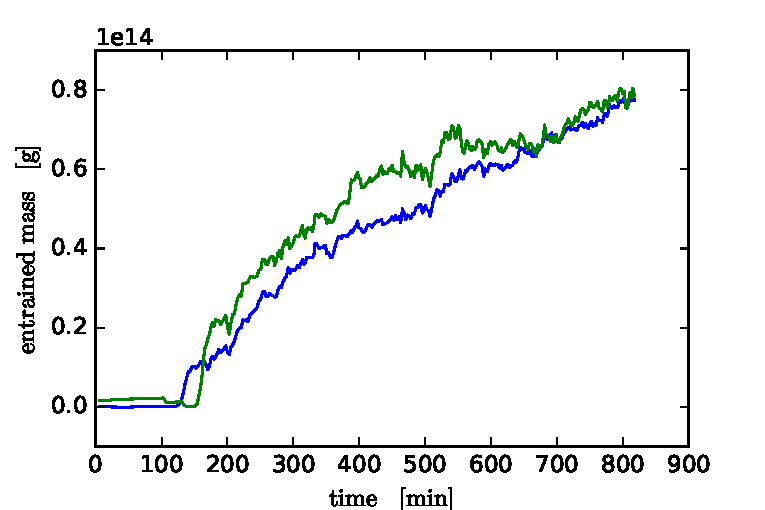
\includegraphics[width=0.5\textwidth]{./img/ent.pdf}\label{fig:ent}}
	\hfill
  \centering
    \subfloat[Turbulence standard deviation over time.]{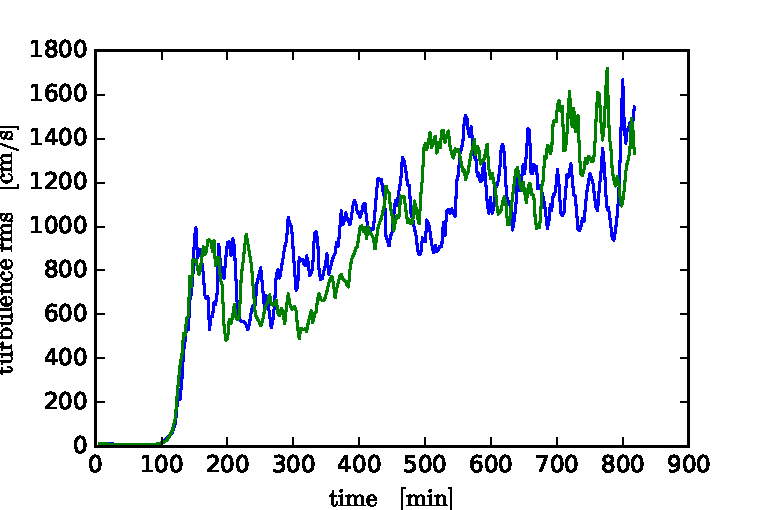
\includegraphics[width=0.5\textwidth]{./img/sigt.pdf}\label{fig:sigt}}
      \hfill
        \subfloat[Turbulence length scale over time.]{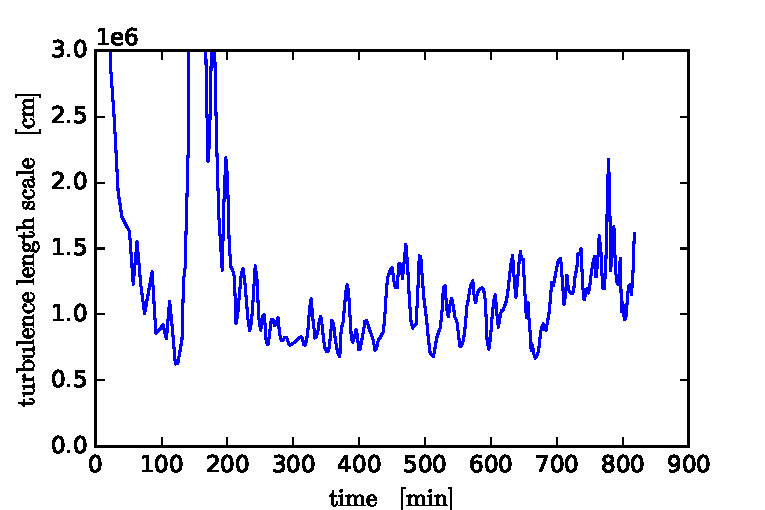
\includegraphics[width=0.5\textwidth]{./img/len.pdf}\label{fig:len}}
	\hfill
  \centering
    \subfloat[Buoyancy jump over time.]{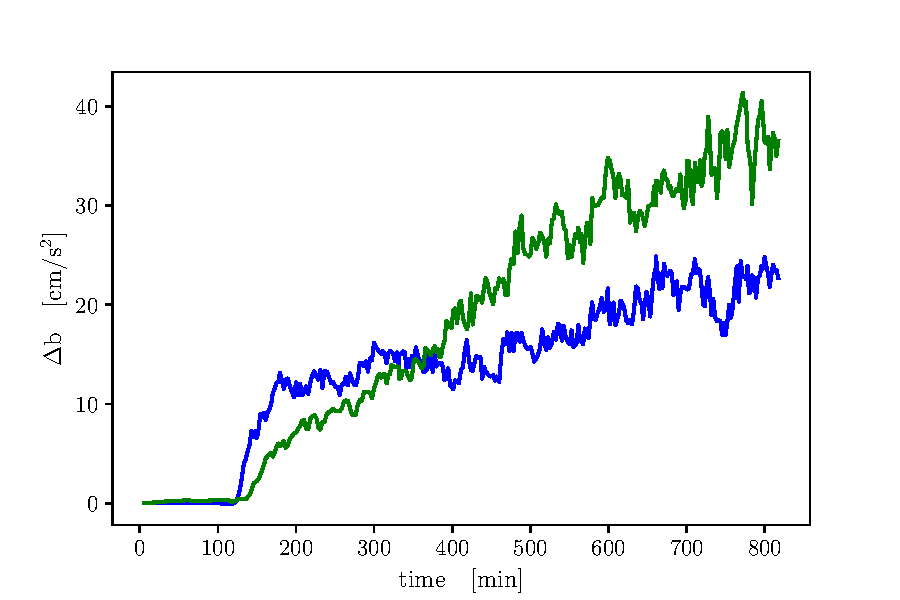
\includegraphics[width=0.5\textwidth]{./img/delb.pdf}\label{fig:delb}}
      \hfill
        \subfloat[Bounday position and width over time. Shaded regions represent the boundary thickness.]{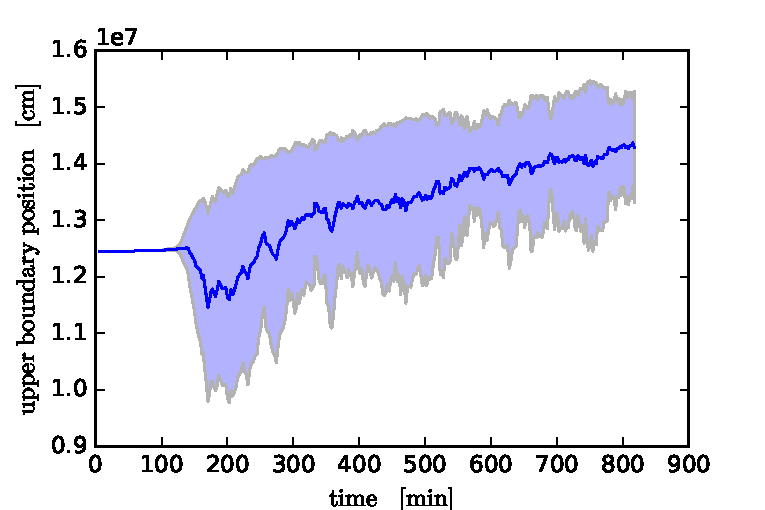
\includegraphics[width=0.5\textwidth]{./img/boundpos.pdf}\label{fig:boundpos}}
	\caption{Plots of the relevant parameters for our analysis over time. Blue lines represent the upper boundary, green lines the lower boundary.}
	  \label{fig:2dsingle}
  \end{figure}
We show first of all the bulk-Richardson number over time. Blue lines represent the upper boundary, green lines lower boundary. At around $t=\mathrm{300 \ min}$, when the entrainment becomes linear, the bulk-Richardson number still oscillates over half an order of magnitude. This obviously deeply affects our data analysis, making necessary a large amount of runs to collect as more data as possible. This also makes impracticable a differential study of the entrainment over time. \\
Second of all we plot in figure \ref{fig:ent} the entrained mass over time. As already mentioned we will perform a Lagrangian study of entrainment, because it is impracticable to quantify how much of the boundary movement is due to the entrained mass or to the adiabatic expansion of the fluid. We notice that also the entrainment rate stabilizes after the initial transition. \\
  In figure \ref{fig:sigt} we plot the turbulence standard deviation over time. It is overall constant, with a slight trend to increase. This result has been obtained after extensive tests to correctly tune the heating function.\\
  In figure \ref{fig:len} we plot the turbulent length scale $L$ over time. In this case we only calculated $L$ at the center of the convective layer, so this value will be used both for the upper and lower boundary analysis. The length scale at the interfaces has a value which is overall comparable, but it is affected by some spikes, reason for which we decided to calculate it in a fully convective region.\\ 
  The last ingredient of the bulk-Richardson number is the buoyancy jump $\Delta b$, that we plot in figure \ref{fig:delb}. In both cases there is an increasing trend, more significant in the lower boundary. This plot shows one of the biggest challenges of running simulation to study differentially the bulk-Richardson number: it is extremely hard to obtain a run where all the parameters ($\Delta b$, $L$, $\sigma_t$ and $M_{\mathrm{E}}$) are constant over time. One finds hence itself in the inconvenient situation of having to average over values that span a full order of magnitude with a strong increasing or decreasing trend, and the quality of the analysis is consequentially affected by this uncertainty.\\
 \begin{figure}[t!]
\centering
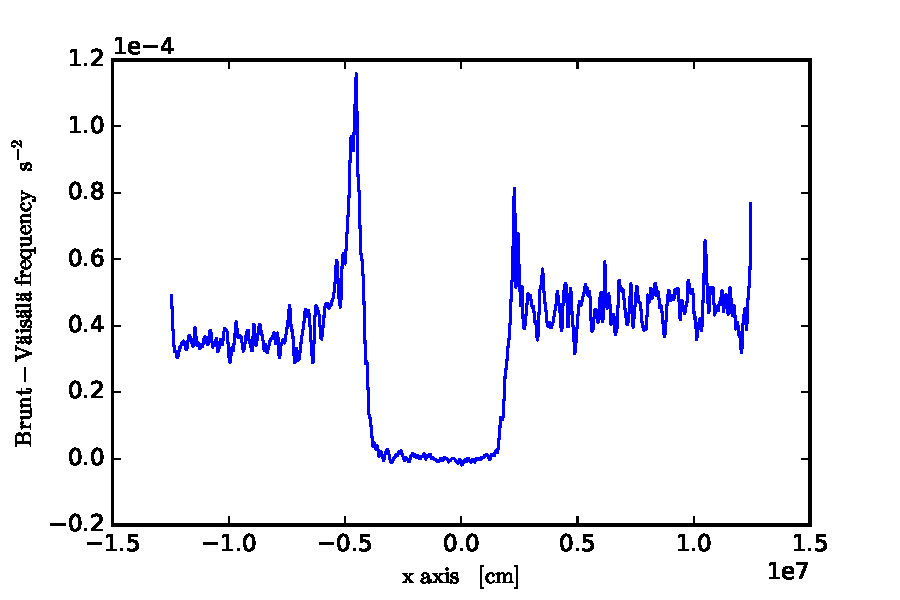
\includegraphics[width=0.5\textwidth]{./img/brunt}
\caption{Horizontal average of the Brunt-Väisälä frequency at about $t=500 \ \mathrm{min}$.}
\label{fig:brunt}
\centering
\end{figure}
For completeness we plot in \ref{fig:boundpos} the boundary position over time. As previously mentioned an Eulerian study is impracticable for this phenomenon, because it is hard to quantify how much of the boundary migration in an Eulerian frame is due to the entrainment and how much due to the adiabatic expansion of the fluid. Nevertheless we would like to point out that, once the entrainment rate stabilizes at $t=300 \ \mathrm{min}$, the boundary thickness is also overall stable in both the upper and lower case. \\
For every 2D or 3D run we will extrapolate the relevant parameters and present them in the following layout
\begin{center}
 \begin{tabular}{l|c|c}
	 Run &2d0.7-0.01U&2d0.7-0.01L\\
	  	\hline
	   $\Delta b$ $(\mathrm{cm/s^{2}})$&$ 9.88 \pm 2.16 $&$18.62 \pm 6.33$\\
		\hline
	   $\sigma_t$ $(\mathrm{cm/s})$ &$ 1127 \pm 169 $&$1185 \pm 231$\\
		\hline
	   $L$ $(\mathrm{cm})$&$(5.47 \pm 1.32) \times 10^5$&$(5.47 \pm 1.32) \times 10^5$\\
		\hline
	   $Ri_{\mathrm{B}}$& $4.487 \pm 1.946 $&$7.268 \pm 2.537$\\
		\hline
	   $\dot{M}_{\mathrm{ent}}$ $(\mathrm{g/s})$ &$(1.338 \pm 0.012) \times 10^9$&$(9.182 \pm 0.024) \times 10^8$\\
      \end{tabular}
 \end{center}
 Where the U at the end of the run name stands for upper boundary, and the L for lower boundary. \\
 Notice that the lower boundary is stiffer than the upper one (the buoyancy jump is higher, and hence the bulk-Richardson number) even if in the initial setup the Brunt-Väisälä frequency is the same for the two stable regions. Looking at figure \ref{fig:brunt} it is clear that at the convective boundaries a spike arises during the simulation in the Brunt-Väisälä frequency, and in the lower case it is more pronounced. Obviously when integrated over the interface, this gives rise to a bigger buoyancy jump.


\subsection{Resolution study}
\begin{figure}[t!]
  \centering
  \subfloat[Mach number profile for the $2048 \times 1024$ run.]{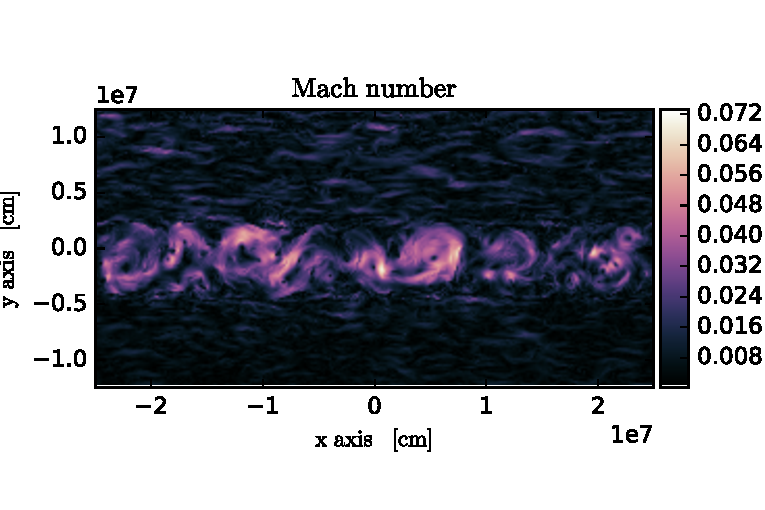
\includegraphics[width=10cm]{./img/machhighres.pdf}}
  \centering
      \hfill
    \subfloat[Mach number profile for the $512 \times 256$ run.]{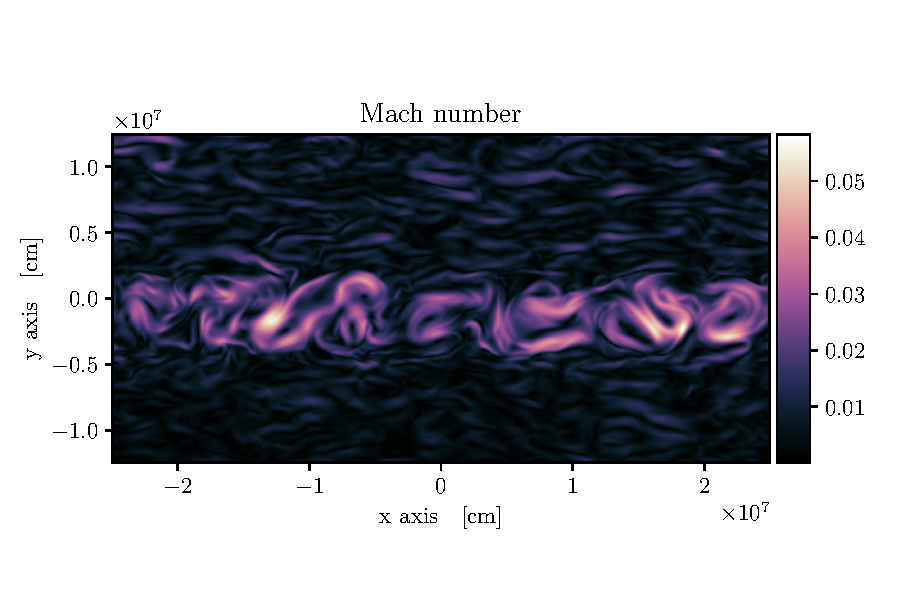
\includegraphics[width=10cm]{./img/machlowres.pdf}}
    \caption{Turbulent structures at different resolutions at about $t=500 \ \mathrm{min}$.}
    \label{fig:differentialmach}
 \end{figure}

In the last section we analysed the run 2d0.10-0.80. What we will do in this section is to compare the previous results with the ones obtained by running the same setup on smaller resolutions, in order to understand if we are properly resolving the system. \\
The same setup was run on a $1024 \times 512$ and $512 \times 256$. As expected, the highest resolution run shows smaller and more refined turbulent structures in the convective region, while in the smallest run we observe less eddies but of bigger size (see figure \ref{fig:differentialmach}).\\
We report in the following table the relevant parameters of the upper boundary for the different resolution runs. We observe that all the parameters are overall constant, within a $10 \%$ oscillation range. Woodward \textit{et al.} \cite{woodward} found that the entrainment rate decreases exponentially with the enhancement of the resolution, before converging to the physical value. In our case we observe a constant entrainment (with a slight increasing trend, we presume due to second order phenomena), and hence we can safely assume that even in the lowest resolution case we are properly resolving the system. One could still point out that the convergence reached in a 2D setup does not imply a convergence in 3D, but being 3D simulations computationally so expensive, it is impracticable for us to test this hypothesis.
\begin{center}
 \begin{tabular}{l|c|c|c}
	 Run &$2048 \times 1024$ U& $1024  \times 512$ U& $512 \times 256$ U\\
	  	\hline
		$\Delta b$ $(\mathrm{cm/s^{2}})$ & $ 8.07 \pm 3.54 $ & $8.18 \pm 1.16$ & $8.28 \pm 0.53$\\
		\hline
		$\sigma_t$ $(\mathrm{cm/s})$ & $ 1118 \pm 202 $ & $1082 \pm 227$ & $1277 \pm 81$\\
		\hline
		$L$ $(\mathrm{cm})$&$(10.88 \pm 2.56) \times 10^5$ & $(11.23 \pm 2.52) \times 10^5$ & $(13.10 \pm 1.07) \times 10^5$\\
		\hline
		$Ri_{\mathrm{B}}$& $8.074 \pm 3.543 $ & $8.495 \pm 3.324 $ & $6.773 \pm 1.277$\\
		\hline
		$\dot{M}_{\mathrm{ent}}$ $(\mathrm{g/s})$ &$(1.287 \pm 0.006) \times 10^9$&$(1.192 \pm 0.013) \times 10^9$ & $(1.132 \pm 0.011) \times 10^9$\\
      \end{tabular}
 \end{center}
Even in the lower boundary all the parameters oscillate within a $10 \%$ range.
\begin{center}
 \begin{tabular}{l|c|c|c}
	 Run &$2048 \times 1024$ L& $1024  \times 512$ L& $512 \times 256$ L\\
	  	\hline
		$\Delta b$ $(\mathrm{cm/s^{2}})$ & $ 8.07 \pm 3.54 $ & $8.18 \pm 1.16$ & $8.28 \pm 0.53$\\
		\hline
		$\sigma_t$ $(\mathrm{cm/s})$ & $ 1118 \pm 202 $ & $1082 \pm 227$ & $1277 \pm 81$\\
		\hline
		$L$ $(\mathrm{cm})$&$(10.88 \pm 2.56) \times 10^5$ & $(11.23 \pm 2.52) \times 10^5$ & $(13.10 \pm 1.07) \times 10^5$\\
		\hline
		$Ri_{\mathrm{B}}$& $8.074 \pm 3.543 $ & $8.495 \pm 3.324 $ & $6.773 \pm 1.277$\\
		\hline
		$\dot{M}_{\mathrm{ent}}$ $(\mathrm{g/s})$ &$(1.287 \pm 0.006) \times 10^9$&$(1.192 \pm 0.013) \times 10^9$ & $(1.132 \pm 0.011) \times 10^9$\\
      \end{tabular}
 \end{center}




\section{Differential study}

\bibliographystyle{mn2e}
\bibliography{./tex/bibliography}
\clearpage
\new{
\chapter*{Acknowledgements}
\thispagestyle{empty}
At this point I need to thank my supervisor Fritz Röpke for welcoming me in the PSO group, suggesting me such an interesting topic to work on and providing a powerful tool as SLH. I need to thank every member of the group for creating such an inspiring and friendly atmosphere. When I walked into my office one year ago, I couldn't have expected any better. In particular I need to thank Philip Edelmann who patiently introduced me in every aspect into the computational universe and Sam Jones for sharing his experience on the CBM problem.

I also feel I need to thank every member of the University of Heidelberg and of the Heidelberg Institute for Theoretical Studies who contributed over the past two years to my academic education.

Furthermore I need to thank the Jülich Supercomputing Center for providing part of the computational resources used for this work.


\clearpage
\setlength{\parindent}{0em}

Erkl\"{a}rung:\par
\vspace{3\baselineskip}
Ich versichere, dass ich diese Arbeit selbstst\"{a}ndig verfasst habe und keine
anderen als die angegebenen Quellen und Hilfsmittel benutzt habe.\par
\vspace{5\baselineskip}
Heidelberg, den (Datum)\hspace{3cm}\dotfill

}
\end{document}
